\def\year{2021}\relax
%File: formatting-instructions-latex-2021.tex
%release 2021.1
\documentclass[letterpaper]{article} % DO NOT CHANGE THIS
\usepackage{aaai21}  % DO NOT CHANGE THIS
\usepackage{times}  % DO NOT CHANGE THIS
\usepackage{helvet} % DO NOT CHANGE THIS
\usepackage{courier}  % DO NOT CHANGE THIS
\usepackage[hyphens]{url}  % DO NOT CHANGE THIS
\usepackage{graphicx} % DO NOT CHANGE THIS
\urlstyle{rm} % DO NOT CHANGE THIS
\def\UrlFont{\rm}  % DO NOT CHANGE THIS
\usepackage{graphicx}  % DO NOT CHANGE THIS
\usepackage{natbib}  % DO NOT CHANGE THIS AND DO NOT ADD ANY OPTIONS TO IT
\usepackage{caption} % DO NOT CHANGE THIS AND DO NOT ADD ANY OPTIONS TO IT
\frenchspacing  % DO NOT CHANGE THIS
\setlength{\pdfpagewidth}{8.5in}  % DO NOT CHANGE THIS
\setlength{\pdfpageheight}{11in}  % DO NOT CHANGE THIS
%\nocopyright
\usepackage{amsfonts}       % blackboard math symbols
\usepackage{amssymb}
\usepackage{bm}
\usepackage{nicefrac}       % compact symbols for 1/2, etc.
\usepackage{microtype}      % microtypography
\usepackage{amsmath}
\usepackage{xcolor}
\usepackage{adjustbox}
\usepackage{multirow}
\usepackage{enumitem}
% \usepackage[normalem]{ulem}
\usepackage[skip=2pt,font=footnotesize,labelfont=bf]{caption}
%PDF Info Is REQUIRED.
% For /Author, add all authors within the parentheses, separated by commas. No accents or commands.
% For /Title, add Title in Mixed Case. No accents or commands. Retain the parentheses.
\pdfinfo{
/Title (AAAI Press Formatting Instructions for Authors Using LaTeX -- A Guide)
/Author (AAAI Press Staff, Pater Patel Schneider, Sunil Issar, J. Scott Penberthy, George Ferguson, Hans Guesgen, Francisco Cruz, Marc Pujol-Gonzalez)
/TemplateVersion (2021.1)
} %Leave this
% Colors
\definecolor{our_blue}{rgb}{0.21747533000128158, 0.5305292836088684, 0.7548225041650647}
\definecolor{our_red}{rgb}{0.7364705882352941, 0.08, 0.10117647058823528}
% /Title ()
% Put your actual complete title (no codes, scripts, shortcuts, or LaTeX commands) within the parentheses in mixed case
% Leave the space between \Title and the beginning parenthesis alone
% /Author ()
% Put your actual complete list of authors (no codes, scripts, shortcuts, or LaTeX commands) within the parentheses in mixed case.
% Each author should be only by a comma. If the name contains accents, remove them. If there are any LaTeX commands,
% remove them.

% DISALLOWED PACKAGES
% \usepackage{authblk} -- This package is specifically forbidden
% \usepackage{balance} -- This package is specifically forbidden
% \usepackage{color (if used in text)
% \usepackage{CJK} -- This package is specifically forbidden
% \usepackage{float} -- This package is specifically forbidden
% \usepackage{flushend} -- This package is specifically forbidden
% \usepackage{fontenc} -- This package is specifically forbidden
% \usepackage{fullpage} -- This package is specifically forbidden
% \usepackage{geometry} -- This package is specifically forbidden
% \usepackage{grffile} -- This package is specifically forbidden
% \usepackage{hyperref} -- This package is specifically forbidden
% \usepackage{navigator} -- This package is specifically forbidden
% (or any other package that embeds links such as navigator or hyperref)
% \indentfirst} -- This package is specifically forbidden
% \layout} -- This package is specifically forbidden
% \multicol} -- This package is specifically forbidden
% \nameref} -- This package is specifically forbidden
% \usepackage{savetrees} -- This package is specifically forbidden
% \usepackage{setspace} -- This package is specifically forbidden
% \usepackage{stfloats} -- This package is specifically forbidden
% \usepackage{tabu} -- This package is specifically forbidden
% \usepackage{titlesec} -- This package is specifically forbidden
% \usepackage{tocbibind} -- This package is specifically forbidden
% \usepackage{ulem} -- This package is specifically forbidden
% \usepackage{wrapfig} -- This package is specifically forbidden
% DISALLOWED COMMANDS
% \nocopyright -- Your paper will not be published if you use this command
% \addtolength -- This command may not be used
% \balance -- This command may not be used
% \baselinestretch -- Your paper will not be published if you use this command
% \clearpage -- No page breaks of any kind may be used for the final version of your paper
% \columnsep -- This command may not be used
% \newpage -- No page breaks of any kind may be used for the final version of your paper
% \pagebreak -- No page breaks of any kind may be used for the final version of your paperr
% \pagestyle -- This command may not be used
% \tiny -- This is not an acceptable font size.
% \vspace{- -- No negative value may be used in proximity of a caption, figure, table, section, subsection, subsubsection, or reference
% \vskip{- -- No negative value may be used to alter spacing above or below a caption, figure, table, section, subsection, subsubsection, or reference
% Colors
\setcounter{secnumdepth}{2} %May be changed to 1 or 2 if section numbers are desired.
\usepackage{booktabs}       % professional-quality tables
% The file aaai21.sty is the style file for AAAI Press
% proceedings, working notes, and technical reports.
%

\usepackage[switch]{lineno}

% Title

% Your title must be in mixed case, not sentence case.
% That means all verbs (including short verbs like be, is, using,and go),
% nouns, adverbs, adjectives should be capitalized, including both words in hyphenated terms, while
% articles, conjunctions, and prepositions are lower case unless they
% directly follow a colon or long dash

\title{Improving Relation Extraction by Leveraging Knowledge Graph Link Prediction}
\author{
    Anonymous
    %Authors
    % All authors must be in the same font size and format.
    % Written by AAAI Press Staff\textsuperscript{\rm 1}\thanks{With help from the AAAI Publications Committee.}\\
    % AAAI Style Contributions by Pater Patel Schneider,
    % Sunil Issar,  \\
    % J. Scott Penberthy,
    % George Ferguson,
    % Hans Guesgen,
    % Francisco Cruz,
    % Marc Pujol-Gonzalez
    \\
}
\affiliations{
    %Afiliations

    % \textsuperscript{\rm 1}Association for the Advancement of Artificial Intelligence\\
    %If you have multiple authors and multiple affiliations
    % use superscripts in text and roman font to identify them.
    %For example,

    % Sunil Issar, \textsuperscript{\rm 2}
    % J. Scott Penberthy, \textsuperscript{\rm 3}
    % George Ferguson,\textsuperscript{\rm 4}
    % Hans Guesgen, \textsuperscript{\rm 5}.
    % Note that the comma should be placed BEFORE the superscript for optimum readability

    % 2275 East Bayshore Road, Suite 160\\
    % Palo Alto, California 94303\\
    % % email address must be in roman text type, not monospace or sans serif
    % publications21@aaai.org

    % See more examples next
}
\iffalse
%Example, Single Author, ->> remove \iffalse,\fi and place them surrounding AAAI title to use it
\title{My Publication Title --- Single Author}
\author {
    % Author
    Author Name \\
}

\affiliations{
    Affiliation \\
    Affiliation Line 2 \\
    name@example.com
}
\fi

\iffalse
%Example, Multiple Authors, ->> remove \iffalse,\fi and place them surrounding AAAI title to use it
\title{My Publication Title --- Multiple Authors}
\author {
    % Authors

        First Author Name,\textsuperscript{\rm 1}
        Second Author Name, \textsuperscript{\rm 2}
        Third Author Name \textsuperscript{\rm 1} \\
}
\affiliations {
    % Affiliations
    \textsuperscript{\rm 1} Affiliation 1 \\
    \textsuperscript{\rm 2} Affiliation 2 \\
    firstAuthor@affiliation1.com, secondAuthor@affilation2.com, thirdAuthor@affiliation1.com
}
\fi

\begin{document}

\maketitle
\linenumbers

\begin{abstract}
Relation extraction (RE) aims to predict a relation between a subject and an object in a sentence, while knowledge graph link prediction (KGLP) aims to predict a set of objects, $O$, given a subject and a relation from a knowledge graph.
These two problems are closely related as their respective objectives are intertwined: given a sentence containing a subject and an object $o$, a RE model predicts a relation that can then be used by a KGLP model together with the subject, to predict a set of objects $O$.
Thus, we expect object $o$ to be in set $O$.
In this paper, we leverage this insight by proposing a multi-task learning approach that improves the performance of RE models by jointly training on RE and KGLP tasks.
We illustrate the generality of our approach by applying it on several existing RE models and achieve new state-of-the-art across several metrics. Moreover, we empirically demonstrate how it helps them achieve consistent performance gains.
\end{abstract}

\section{Introduction}
\label{sec:intro}
Many real-world applications ranging from search engines to conversational agents rely on the ability to uncover new relationships from existing knowledge.
Relation extraction (RE) and knowledge graph link prediction (KGLP) are two learning tasks that are both very popular and that center around inferring new information from existing facts.
RE is a textual inference task that aims to discover the relationship between two entities (termed the subject and the object, respectively) in a sentence.
For instance, given the sentence ``\texttt{Miami is in Florida}'' with subject \texttt{Miami} and object \texttt{Florida}, RE methods have to predict the relationship \texttt{locatedIn}.
RE is important because it is used for downstream applications (e.g., knowledge graph [KG] population) and the underlying ideas are also applicable to other related important problems such as question answering. Knowledge graph link prediction (KGLP), on the other hand, aims to populate KGs by uncovering the set of correct answers (i.e., objects) to questions comprised of graph nodes (i.e., subjects) and edges (i.e., relations) in the form of \texttt{(subject,relation,?)} triples.
The uncovered answers are used to populate the KG by establishing connections between subjects and objects using relations.
For instance, the answers \texttt{Florida} and \texttt{USA} to the question \texttt{(Miami,LocatedIn,?)}, form two new connections in the KG: \texttt{(Miami,LocatedIn,Florida)} and \texttt{(Miami,LocatedIn,USA)}, respectively.

Relation extraction and knowledge graph link prediction are inherently related.
To illustrate, let $s$, $o$ and $r$ represent the subject, object, and relation, respectively, that are contained in a sentence.
RE methods infer the relation $r$ given the sentence, the subject $s$, and the object $o$.
Comparatively, KGLP methods utilize $r$ and $s$ to predict a set of objects $O$ that is expected to include $o$. In our previous examples, $O$ \texttt{= \{Florida, USA\}} and $o$ \texttt{= Florida}, respectively.

Several methods have been proposed to boost the performance of RE models by jointly training over both RE and KGLP tasks.
% Both RE and KGLP have garnered substantial interest and popularity in recent years, and several methods have been proposed to boost the performance of RE methods with the additional supervision of a KGLP model.
% proposed to utilize the additional supervision provided by a KGLP method to boost the performance of a RE model.
% Both RE and KGLP have garnered substantial interest and popularity in recent years, and many method have been proposed to leverage their similarities to improve performance by jointly training over both tasks.
% Both RE and KGLP have garnered substantial interest and popularity in recent years, and several methods have been proposed to leverage their similarities to improve performance by jointly training over both tasks.
However, these approaches typically require KGLP pre-training \citep[e.g.]{weston-2013, lfds}, exhibit constrained parameter sharing \citep[e.g.]{weston-2013, lfds}, or predominately attend over both problems through custom attention mechanisms \citep[e.g.,][]{bag_re_kglp,han,long_tail}.
% While both RE and KGLP have garnered substantial interest and popularity in recent years, less work leverages the aforementioned relationship between the two. 
% We propose a method that leverages this relationship and manages to improve RE performance, by using knowledge acquired while learning to do well on the KGLP task.
% To illustrate the similarities between RE and KGLP, 
% Leveraging additional supervision encapsulated in KGs to improve the performance of RE models has previously been explored by using KGLP methods to {\em fact-check} (i.e., to determine the correctness of the resulting subject-relation-object triple).
% While both RE and KGLP have garnered substantial interest and popularity in recent years, less work leverages
% work has been proposed that attempts to leverage 
% the aforementioned relationship between the two. 
% We propose a method that does exactly that, and also manages to outperform existing methods. but before we summarize our contribution, let us explain what we mean when we say that the two tasks are similar.
% RE predictions \citep[e.g.,][]{weston-2013}.
% While such methods have achieved strong performance, they typically require KGLP pre-training and only allow for very limited information sharing between the two tasks.
% This is because the RE model cannot use any information provided by the KGLP model while producing a ranked list of predictions.
% The KGLP model effectively only acts as a {\em reranker} for the ranked list that the RE model generates.
% Moreover and perhaps most importantly, these methods are not generalizable to arbitrary KGLP models as they are often designed around a specific class of KGLP approaches, 
% nor do they necessarily
% I want to say:
% - previous approaches 
% While such methods have achieved strong performance, they typically require KGLP pre-training, and predominately explicitly attend over both tasks through complicated dual attention mechanisms \citep[e.g.,][]{bag_re_kglp,han,long_tail}.
% and are incapable of reasoning over more expressive recent link prediction approaches.
% Although some prior methods also reason over RE and KGLP problems without using such attention mechanisms, they have to trade-off of very limited information sharing between the two tasks (e.g. \cite{weston-2013}), or learning a single task at a time (e.g. \cite{weston-2013, lfds}).
Although some prior methods also reason over RE using KGLP without such attention mechanisms, they either severely restrict information sharing between the two tasks \citep[e.g.,][]{weston-2013}, or only learn a single task at a time \citep[e.g.,][]{lfds,weston-2013} rather than learning both tasks jointly.
Moreover, these frameworks only support a limited class of KGLP models that can be reframed as inferring relations from subject and objects.
This constraint excludes recent KGLP methods which perform significantly better, but cannot be reformulated to satisfy the restriction.
An ideal framework should support arbitrary RE and KGLP methods, including the significantly more expressive and stronger performing recent KGLP approaches.
Additionally, such a framework should enable RE models to benefit from KGLP models with minimal changes to the underlying RE and KGLP methods.

\begin{figure*}[t]
    \centering
    % \includegraphics[width=1.0\textwidth]{images/coper_horizontal.pdf}
    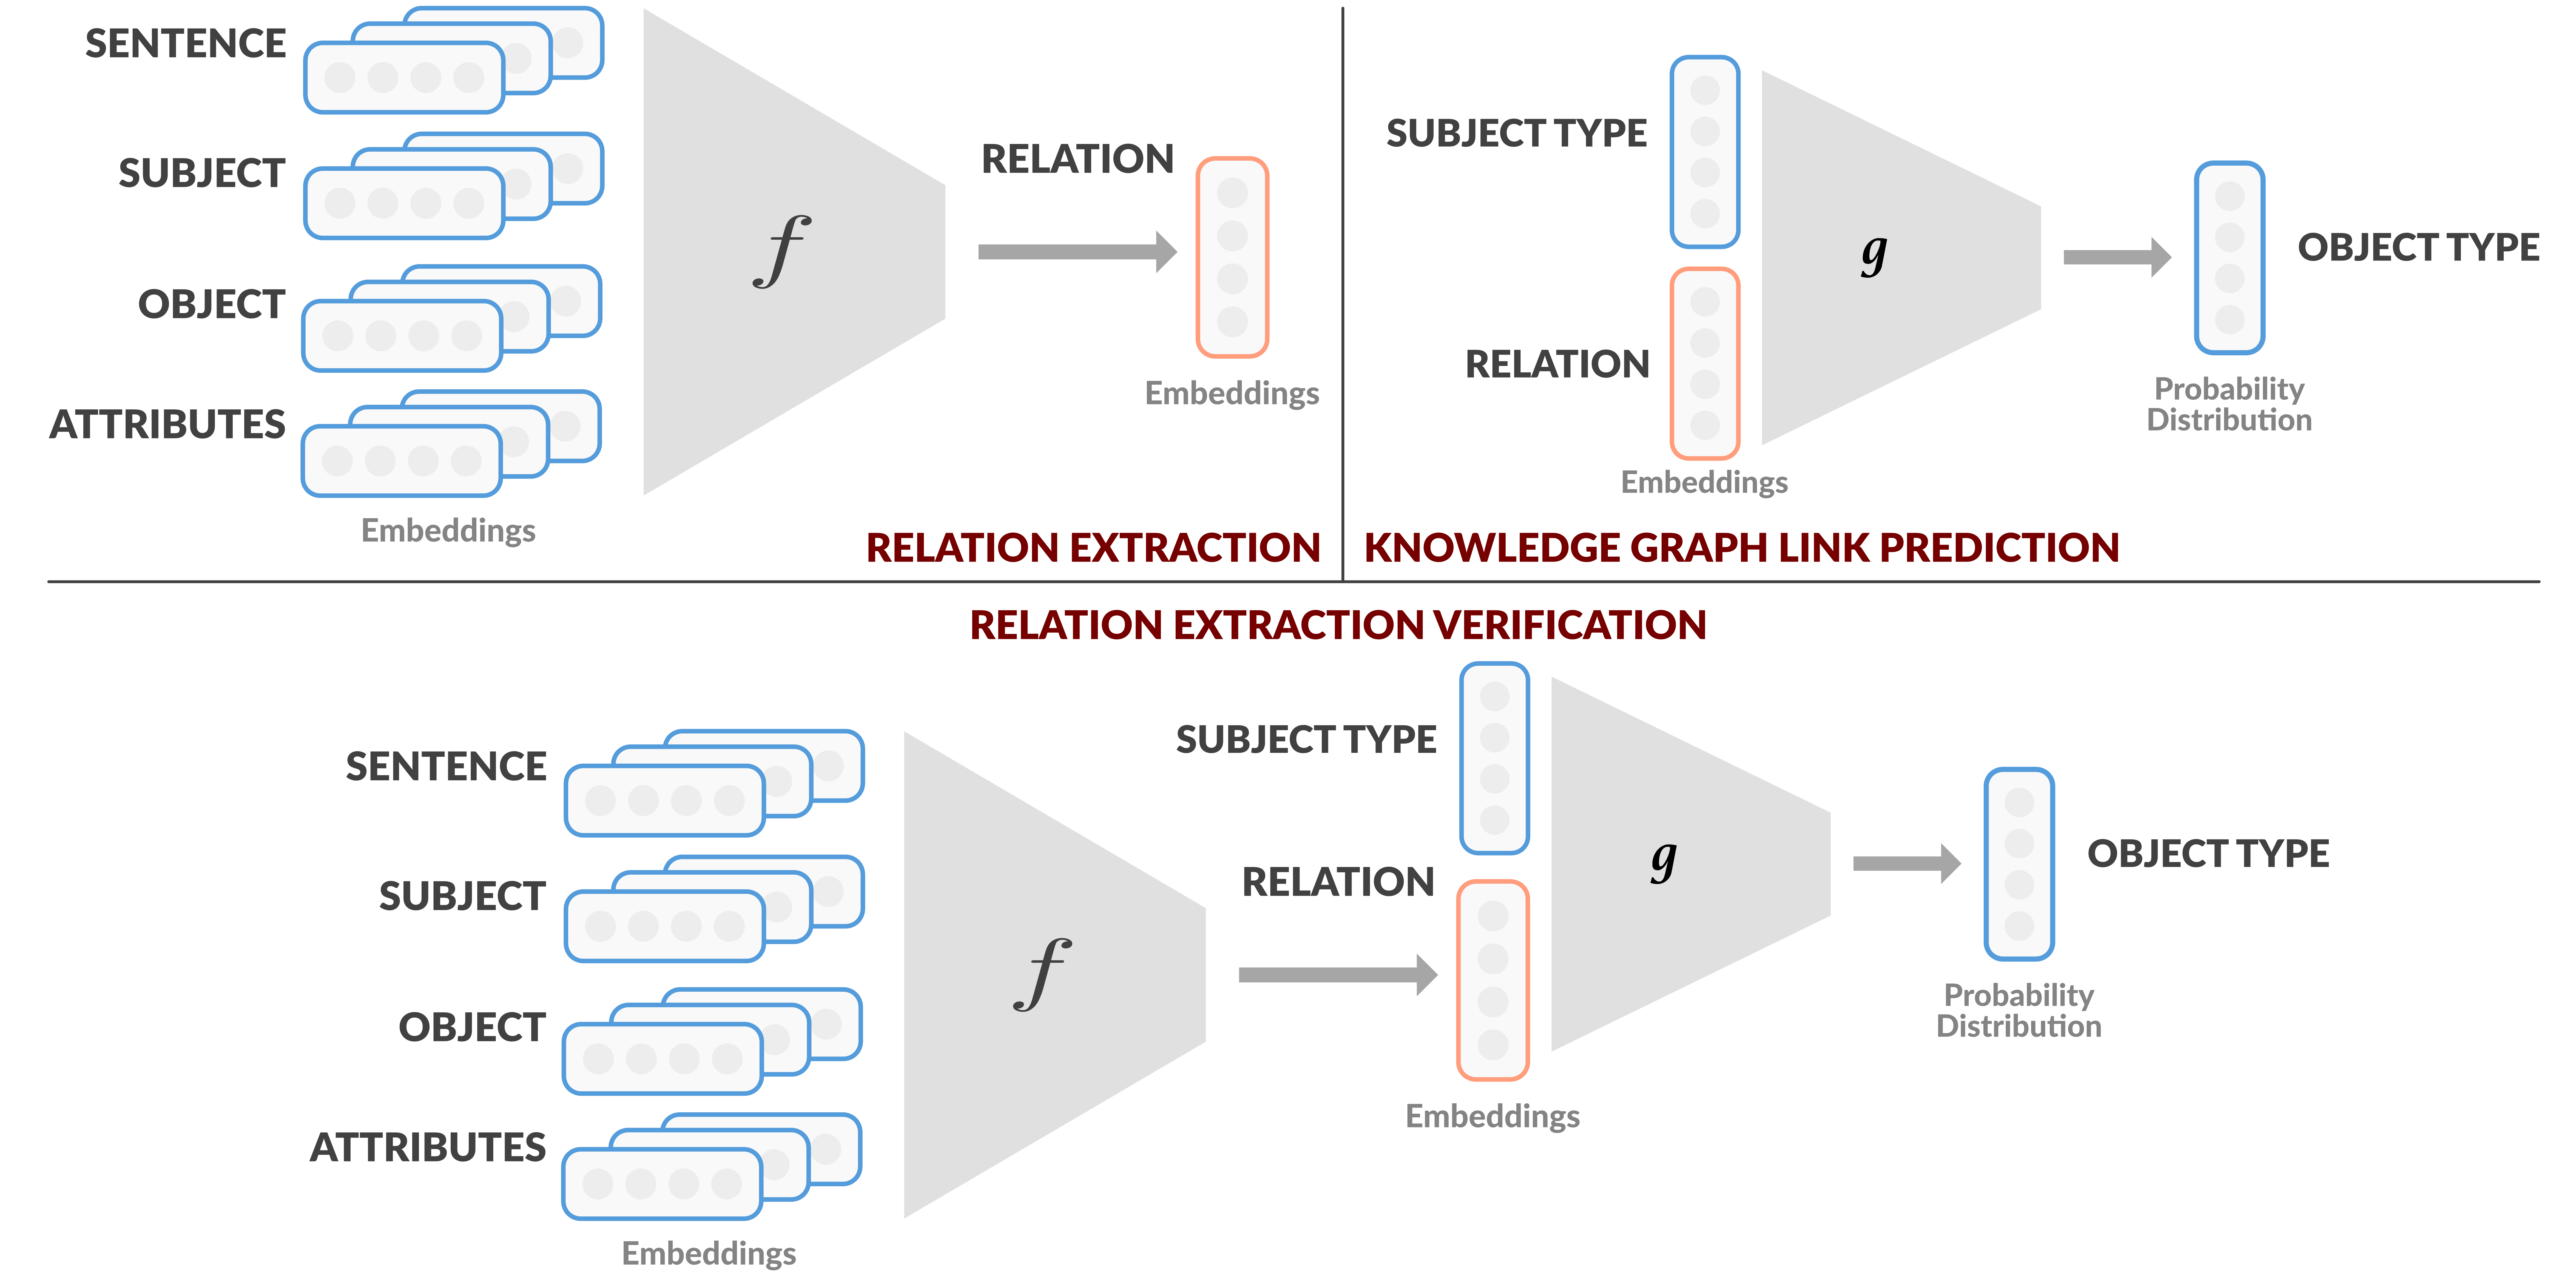
\includegraphics[width=\textwidth]{images/JRELP_figure.png}
    \caption{
        % \eapcomment{TODO: I'm hoping I'll get some time to make an overview figure / modify this one.}
        Overview of JRRELP.
        JRRELP is comprised of three loss terms: the RE loss, the KGLP loss, and the coupling loss.
        The RE loss is illustrated in the top-left quadrant, the KGLP loss is described by the top-right quadrant, and the bottom half shows the coupling loss.
        % The first task, relation extraction, is illustrated in the top-left quadrant. There, a RE model infers a relation between a sentence subject and object, given the two components, and additional sentence attributes and sentence. The second task of knowledge graph link prediction is visualized in the top-right quadrant. Given a relation and subject type -- obtained via subject {\em type-substitution}, the objective is to predict the a set of object types. Lastly, the bottom half exhibit the third task of RE verification. Similar to the second task, an RE model's relation prediction is utilized in place of the pre-existing relation to infer the set of object types.
        }
    \label{fig:JRRELP-overview}
    % \vspace{-4ex}
\end{figure*}

% Moreover, these approaches are also limited to specific KGLP model classes.

% Moreover and perhaps most importantly, these methods are not generalizable to arbitrary KGLP models as they are often designed around a specific class of KGLP models, nor do they necessarily support a broad .

% In an ideal setting, we would expect any RE model to be able to benefit from a strong KGLP model.
We propose a general framework which ties the RE and KGLP tasks cohesively into a single learning problem.
Our architecture, termed \textbf{JRRELP}---\textbf{J}ointly \textbf{R}easoning over \textbf{R}elation \textbf{E}xtraction with \textbf{L}ink \textbf{P}rediction---has the following desirable properties:
\begin{itemize}[noitemsep,topsep=0pt,label=--,leftmargin=2em]
  \item \textbf{Generality:}
    Our method can be applied to arbitrary RE and KGLP models to boost RE performance.
    % Our method can be applied to arbitrary RE and KGLP models to boost their performance.
    The only assumption JRRELP makes is that both models are trained by minimizing a loss function (which is common across all successful RE and KGLP methods).
  \item \textbf{Effective Information-Sharing:}
    JRRELP introduces a {\em cyclical} relationship between model parameters, enabling better information transfer between the learning tasks.
    Moreover, {\em all} parameters are shared across both the RE and KGLP tasks.
    % RE and KGLP task parameters, and 
    % In JRRELP, the model parameters used for RE and KGLP are {\em all} shared, enabling better information transfer between the tasks. Moreover, JRRELP establishes a novel cyclical relationship between task parameters. 
    % To the best of our knowledge, this is not true for prior work.
  \item \textbf{Performance:}
    % JRRELP boosts the performance of all baseline methods that we used in our evaluation, and achieves a new state-of-the-art. 
    JRRELP boosts the performance of all baseline methods used in our evaluation, and achieves state-of-the-art performance.
    Additionally, JRRELP-enhanced baselines even match or improve upon the performance of more expressive RE models.
    For example, we are able to train C-GCN \citep{cgcn} to match TRE \citep{tre}, even though the latter was proposed as a stronger and significantly more expressive alternative.
  \item \textbf{Efficiency:}
    JRRELP does not require any task-specific pre-training.
    It introduces a minimal overhead over the baseline methods (only $6\%$ slower per mini-batch).
    % JRRELP streamlines model training by not requiring any task-specific pretraining.
    % In JRRELP, both RE and KGLP problems are trained jointly without any task-specific pre-training, reducing training time over previous approaches \citep[e.g.,][]{han,lfds,weston-2013}.
\end{itemize}
% Additionally, JRRELP enhances the performance of weaker baselines to match that of stronger and more expressive models. For instance, applying JRRELP over C-GCN\citep{cgcn} enables it to match TRE \citep{tre}, despite the fact that TRE was proposed as a stronger and significantly more expressive alternative RE model.
% Finally, we also made an interesting observation in our experiments. 
% JRRELP on can enhance the performance of weaker baselines to match that of stronger and more expressive models.
% For example, we are able to train C-GCN \citep{cgcn} to match TRE \citep{tre}, even though the latter was proposed as a stronger and significantly more expressive alternative.
% This is explained in detail in Section~\ref{sec:experiments}.
An overview of JRRELP is shown in Figure~\ref{fig:JRRELP-overview}, and is explained in detail in Section~\ref{sec:JRRELP}.
Next, we present our proposed method and defer positioning with respect to related work until Section~\ref{sec:related_work}.


\section{Background}
\label{sec:background}
% In this section, we describe our method, its learning tasks, and the notation used throughout the paper.

% Before describing our proposed method, we present our notation, and clear definitions of the relevant learning tasks and models.
% Before describing our proposed method, we introduce the notation and tasks 

Before presenting our method, we introduce the notation used throughout this paper, and describe the relevant learning tasks.
% \subsection{Notation}
% \label{sec:data}
% Our main motivation and focus for this work is to perform well in the RE task.
% Therefore, our training data $\mathcal{D}$ contains a collection of sentences.
Let $\mathcal{D}$ describe a dataset that contains a collection of sentences.
Let $X=[x_1, x_2, \ldots x_n]$ denote a sentence, where $x_i$ represents a one-hot encoding for the $i^{\text{th}}$ sentence token (i.e., word).
Each sentence contains a subject $s = [x_{s^{\textrm{start}}}, x_{s^{\textrm{start}} + 1}, \hdots, x_{s^{\textrm{end}}}]$, that is defined as a contiguous span $(s^{\textrm{start}}, s^{\textrm{end}})$ over the sentence, and an object $o = [o_{o^{\textrm{start}}}, o_{o^{\textrm{start}} + 1}, \hdots, o_{o^{\textrm{end}}}]$, that is similarly defined.
Subjects and objects are summarized by their {\em types}, termed $s^{\textrm{type}}$ and $o^{\textrm{type}}$, respectively.
If not already given, these can be extracted by widely used parsing frameworks such as \citep{stanfordcorenlp}.
% A {\em type} is also provided for each such subject/object span and termed $s^{\textrm{type}}$ and $o^{\textrm{type}}$ respectively.
For example, consider the sentence ``\texttt{\textcolor{our_blue}{John Doe} lives in \textcolor{our_red}{Miami}}'', where the subject is shown in \textcolor{our_blue}{blue} color and the object in \textcolor{our_red}{red} color.
In this case, the subject may be tagged as having type \textcolor{our_blue}{\texttt{PERSON}} and the object may be tagged as having type \textcolor{our_red}{\texttt{CITY}}.
Several methods \citep[e.g.,][]{palstm, cgcn, aggcn} employ {\em type-substitution} during data preprocessing: substituting subjects and objects in sentences with their corresponding types.
% During data preprocessing , subjects and objects may be substituted with their corresponding types. 
For instance, with type-substitution our example sentence becomes
% For instance, the example sentence becomes
``\texttt{\textcolor{our_blue}{SUBJECT-PERSON SUBJECT-PERSON} lives in \textcolor{our_red}{OBJECT-CITY}}.''
% Following prior literature \citep{palstm, cgcn, aggcn}, we assume that sentences are preprocessed using type-substitution for the remainder of this paper.
For ease of future explanation, we assume that sentences are preprocessed using type-substitution for the remainder of this paper.
% During data preprocessing, all subject and object tokens in sentences are substituted with their corresponding types.
% For the aforementioned example, the sentence after preprocessing becomes ``\texttt{\textcolor{our_blue}{SUBJECT-PERSON SUBJECT-PERSON} lives in \textcolor{our_red}{OBJECT-CITY}}.''
% We refer to this as {\em type-substitution}.
% We refer to this preprocessing step as {\em type-substitution} and note that it is a relatively standard preprocessing step for this task that is used by \citet{palstm}, \citet{cgcn}, and \citet{aggcn}.
Each sentence may contain additional structural features such as part-of-speech (POS) tags, named-entity-recognition (NER) tags, and a dependency parse. Analogous to extracting entity types, these can be generated from parsing frameworks. 
We denote all such sentence features as members of a set $C$.
% Additionally, each sentence may contain more structural information features such as part-of-speech (POS) and named entity recognition (NER) tags, as well as a dependency parse.
% We shall denote all such features associated with a sentence $X$ as a set $C$.
Finally, each sentence contains a relation, $r$, between its subject and object. 
This may either describe their lack of connection (via a special \texttt{no-relation} token), or an existing one.
% Finally, for each sentence we also have an associated relation $r$ that the sentence describes.
For instance, the relation between \textcolor{our_blue}{\texttt{John Doe}} and \textcolor{our_red}{\texttt{Miami}} in our example sentence would be \texttt{LivesIn}.
% In the aforementioned example, the relation could be \texttt{livesIn}.
In summary, $\mathcal{D}$ is a set of $N$ tuples: $\mathcal{D} = \{ ( X_i, C_i, s_i, o_i, s^{\textrm{type}}_i, o^{\textrm{type}}_i, r_i ) \}_{i=1}^N$, where $N$ is the number of sentences.

\subsection{Relation Extraction}
\label{sec:re-task}

Relation extraction (RE) uses $X$, $C$, $s$, and $o$ from $\mathcal{D}$ to infer the relation $r$ between $s$ and $o$.
Many successful RE methods---including the current state-of-the-art \citep{bert-em}---involve learning vector embeddings for each component.
% Most successful models that have been proposed to tackle this task---including the current state-of-the-art \citep{bert-em}---involve learning vector embeddings for each component.
Specifically, let $N_v$, $N_r $, and $N_c$ denote the vocabulary size for sentence tokens, the number of unique relations, and the number of unique attributes in $C$, computed over the whole training dataset.
Additionally, let $D_v$, $D_r $, and $D_c$ denote the corresponding embedding sizes.
We define $\bm{V}\in\mathbb{R}^{D_v\times N_v}$, $\bm{R}\in\mathbb{R}^{D_r\times N_r}$, and $\bm{A}\in\mathbb{R}^{D_c\times N_c}$ as the vocabulary, relation, and attribute embedding matrices, respectively.
Note that $\bm{V}, \bm{R}$, and $\bm{A}$ are learnable model parameters.
Given a sentence, a subject, an object, and its attributes, their respective embedding representations are defined as:
$\bm{X} = \bm{V}X \in \smash{\mathbb{R}^{D_v \times n}}$,
$\bm{C} = \bm{A}C \in \smash{\mathbb{R}^{D_c\times c}}$,
$\bm{s} = \bm{V}s \in \smash{\mathbb{R}^{D_v \times (s^{\textrm{end}} - s^{\textrm{start}} + 1)}}$, and
$\bm{o} = \bm{V}o \in \smash{\mathbb{R}^{D_v \times (o^{\textrm{end}} - o^{\textrm{start}} + 1)}}$,
where $n$ is the number of tokens in $X$ and $c$ is the number of attributes in $C$.
Similarly, we define the embedded relation as $\bm{r} = \bm{R}r \in \mathbb{R}^{D_r}$.
Given these embeddings, most successful RE models \citep[e.g.,][]{palstm,cgcn,aggcn,tre,bert-em} can be formulated as instances of the following model:

\begin{align}
    & \bm{X} = \bm{V}X,\;
      \bm{C} = \bm{A}C,\;
      \bm{s} = \bm{V}s,\;
      \bm{o} = \bm{V}o \\
    %   ,
    % && \textsc{\sffamily\scriptsize\textcolor{gray}{EMBEDDING}} \\
    & \hat{\bm{r}} = f(\bm{X}, \bm{C}, \bm{s}, \bm{o}) \\
    % ,
    % && \textsc{\sffamily\scriptsize\textcolor{gray}{PREDICTION}} \\
    & p(r \mid \hat{\bm{r}}) = \textrm{Softmax}(\bm{R}\hat{\bm{r}} + \bm{b})
    % ,
    % && \textsc{\sffamily\scriptsize\textcolor{gray}{PROBABILITY ESTIMATION}}
    \label{eq:re-model}
\end{align}
where $\hat{\bm{r}}$ is the inferred relation representation from a prediction model $f$.
% A probability distribution over relations is constructed by applying the ``Softmax'' function over the sum of the dot-product between $\hat{\bm{r}}$ and the relation embeddings $\bm{R}$, and a learnable bias term $\bm{b} \in \mathbb{R}^{N_r}$.
To demonstrate how multiple RE methods fit under this formulation, we briefly describe the three baseline models used in our experiments.
% In order to demonstrate how multiple RE methods fit under this formulation, we now provide a brief description of the two baseline methods used in our experiments.

\textbf{PA-LSTM.}
This model was proposed by \citet{palstm}, and centers around formulating $f$ as the combination of a one-directional long short-term memory (LSTM) network, and a custom position-aware attention mechanism.
The sentence attributes it uses are POS and NER tags, as well as SO and OO tags representing the positional offset of each token from the subject and the object respectively. The method first applies the LSTM over the concatenated sentence, POS tag, and NER tag embeddings. A relation $\hat{\bm{r}}$ is then predicted by attending the LSTM outputs with a custom position-aware attention mechanism using the SO and OO tag embeddings.
% For further details, we refer readers to the work of \cite{palstm}.
% Under our abstract formulation, the PA-LSTM model is defined by using a particular instance of the $f$ function that centers around a long short-term memory \citep[LSTM;][]{lstm} network.
% Specifically, $f$ comprises of first concatenating the sentence and the POS and NER tag embeddings and then applying a one-directional LSTM network over the resulting sequences.
% The outputs of this LSTM are attended over using the SO and OO tag embeddings, by applying a custom position-aware attention mechanism.
% For further details, we refer readers to the work of \cite{palstm}.

\textbf{C-GCN.}
This model was proposed by \citet{cgcn}, and formulates $f$ as a graph-convolution network (GCN) over sentence dependency parse trees. It uses the same sentence attributes as PA-LSTM, and additionally the sentence dependency parse.
Similar to PA-LSTM, the method first encodes a concatenation of the sentence, POS tag, and NER tag embeddings using a bi-directional LSTM network. The model then infers relations from these encodings by reasoning over the graph implied by a pruned version of the provided dependency tree parse.
% and is one of the best performing RE models.
% The sentence attributes it uses are POS tags, NER tags, and a sentence dependency parse, as well as SO and OO tags.
% Similar to the PA-LSTM, the sentence embeddings are concatenated with their respective POS and NER tag embeddings, and encoded using bi-directional LSTM network.
% However, in contrast to PA-LSTM, C-GCN infers relations from these encodings by reasoning over the graph implied by a pruned version of the provided dependency parse tree.
In particular, C-GCN computes the least common ancestor (LCA) between $s$ and $o$, and uses the SO and OO tags to prune the tree around the LCA.
Afterwards, C-GCN processes the sentence encodings using a graph convolution network (GCN) defined over the pruned dependency parse tree.
The resulting representations are finally processed by a multi-layer perceptron to predict relations.
% For further details, we refer readers to the work of \cite{cgcn}.

\textbf{SpanBERT.} 
This model was proposed by \citet{spanbert}, and is one of the current state-of-the-art (SoTA) relation extraction methods.
SpanBERT differs form BERT in that it is pre-trained at the span-level.
Moreover, the model randomly masks contiguous text spans instead of individual tokens, and adds a span-boundary objective that infers masked spans from surrounding data.
In contrast to PALSTM and C-GCN, SpanBERT only takes into account the type-substituted sentence in its input to predict relations.
We chose this model because it is one of the current state-of-the-art RE models and it is also open-sourced, allowing to easily integrate it in our experimental evaluation pipeline.

Note that PA-LSTM, C-GCN, and SpanBERT are just three of many approaches supported by our abstract RE model formulation.
For instance, more other transformer-based methods \citep{tre,bert-em,knowbert} can also be represented by using a different definition for $f$.

\subsection{Knowledge Graph Link Prediction}
\label{sec:kglp-task}

The objective in knowledge graph link prediction (KGLP) is to infer a set of objects $O$ given a question, $(s, r, ?)$, in the form of a subject-relation-object triple, missing the object.
Typically, $s$ and $o$ are nodes in a knowledge graph (KG), while $r$ represents a graph edge.
Although $\mathcal{D}$ does not necessarily provide an explicit KG to reason over, it is possible to generate one by assigning unique identifiers for all subjects, relations, and objects, For instance, these may be $s^{\textrm{type}}$ and $o^{\textrm{type}}$ for subjects and objects respectively, and the relation itself.
Although we assume that these identifiers are used 
(as they are available in our training data $\mathcal{D}^{\textrm{train}}\subset \mathcal{D}$)
for the remainder of this paper, we emphasize that our method is not limited to datasets with these characteristics. Instead our framework supports any $\mathcal{D}$ that specifies a mapping to a pre-existing KG, or where it is possible to define other unique identifiers. This is a very weak constraint.
% unique subject, relation, and object identifiers, which is a very weak constraint. 
% While our training data does not necessarily provide an explicit KG to reason over, it is possible to generate one by assigning unique identifiers for all subjects, relations, and objects.
% For instance, these may be defined as their corresponding types.
% Note that given subject and object types we can ``infer'' relation types as the pair of subject and object types that they appear with in the training data.
% In what follows we assume that types are used as the identifiers (as they are available in our training data), but we want to emphasize that our method is not limited to datasets with these characteristics; it instead supports any dataset that specifies a mapping to a pre-existing KG, or where it is possible to define unique subject, relation, and object identifiers, which is a very weak constraint.
Therefore, given a sentence with $s$, $o$, and $r$, we can use the subject and object types---$s^{\textrm{type}}$ and $o^{\textrm{type}}$, respectively---to form a KG whose edges are represented by each $r$ and nodes by each $s^{\textrm{type}}$ and $o^{\textrm{type}}$.
% Furthermore, we can also include relations $\hat{r}$ predicted by an RE method as additional edges between $s^{\textrm{type}}$ and $o^{\textrm{type}}$.
For ease of notation, we assume that each term is a one-hot encoding of the corresponding identifier.

Due to the {\em type-substitution} preprocessing step described in Section~\ref{sec:background}, all types are included in the sentence token vocabulary.
Thus, we obtain KG component embeddings by:
% We can thus obtain embeddings similar to how we did for the RE task in Section~\ref{sec:re-task}: 
$\bm{s^{\textrm{type}}} = \bm{V} s^{\textrm{type}} \in \smash{\mathbb{R}^{D_v}}$,
$\bm{o^{\textrm{type}}} = \bm{V} o^{\textrm{type}} \in \smash{\mathbb{R}^{D_v}}$, and
$\bm{r} = \bm{R} r \in \smash{\mathbb{R}^{D_r}}$.
Multiple existing KGLP methods can be characterized in terms of the following abstract model:
\begin{align}
    & \bm{s^{\textrm{type}}} = \bm{V} s^{\textrm{type}},\;
      \bm{r} = \bm{R} r \\
    %   ,
    % && \textsc{\sffamily\scriptsize\textcolor{gray}{EMBEDDING}} \\
    & \bm{z} = g(\bm{s^{\textrm{type}}}, \bm{r}) \\
    % ,
    % && \textsc{\sffamily\scriptsize\textcolor{gray}{MERGE}} \\
    & p(O \mid o^{\textrm{type}}, \bm{z}) = \sigma(\bm{V}_{o^{\textrm{type}}}\bm{z} + \bm{b})
    % ,
    % && \textsc{\sffamily\scriptsize\textcolor{gray}{PROBABILITY ESTIMATION}}
    \label{eq:kglp-model}
\end{align}
where $\bm{z}$ is a merged representation of $\bm{s^{\textrm{type}}}$ and $\bm{r}$, and $\sigma$ is the Sigmoid activation function.
% A probability distribution over possible objects is constructed by applying the ``Sigmoid'' function over the sum of the dot-product between $\bm{z}$ and the available object embeddings $\bm{V}_{o^{\textrm{type}}}$, and a learnable bias term $b \in \mathbb{R}^{N_o}$.
Note that the set of available object embeddings $\bm{V}_{o^{\textrm{type}}} \subset \bm{V}$ contains {\em only} valid (in the type-checking sense) object embeddings.
Previous work \citep{coper} shows that multiple KGLP methods fit under this formulation. 
While certain early KGLP methods \citep{bordes2013translating, yang2015embedding, transr_ctranr, transd, trouillon2016complex} do not fit under this formulation, we note that they may be accommodated by a simple reformulation of Equation~\ref{eq:kglp-model} to their respective scoring terms.
We now provide the definition of ConvE \citep{dettmers2018conve} under this formulation, because we use ConvE as our KGLP model in our experiments.
While we acknowledge that ConvE is not the current state-of-the-art (SoTA) KGLP approach, it performs very well while using only a fraction of the parameters current SoTA \cite{coper, GAAT} methods require, thus making it more efficient.
Moreover, ConvE is an example of a KGLP method which cannot be restructured to infer $r$ from $s$ and $o$, making it infeasible to use with any of the previous joint RE and KGLP frameworks \citep[e.g.,][]{lfds,weston-2013}.
Note that, our results can only be further enhanced by using a stronger KGLP approach and thus this choice should not affect our conclusions.

\textbf{ConvE.}
ConvE is defined by using the following merge function in our abstract model formulation:
\begin{align}
    & g(\bm{s^{\textrm{type}}}, \bm{r}) = \text{Conv2D}(\text{Reshape}([s^{\textrm{type}}; \bm{r}])
    % ,
    % && \textsc{\sffamily\scriptsize\textcolor{gray}{MERGE}}
\end{align}
where ``Conv2D'' is a 2D convolution operation and ``$\text{Reshape}([s^{\textrm{type}}; \bm{r}])$'' first concatenates $s^{\textrm{type}}$ and $\bm{r}$ and then reshapes the resulting vector to be a square matrix, so that a convolution operation can be applied to it.
% For further details, we refer readers to \cite{dettmers2018conve}.

\section{Proposed Method}
\label{sec:method}
% In this section, we describe our method, its learning tasks, and the notation used throughout the paper.

% % Before describing our proposed method, we present our notation, and clear definitions of the relevant learning tasks and models.

% \subsection{Notation}
% \label{sec:data}

% Our main motivation and focus for this work is to perform well in the RE task.
% Therefore, our training data $\mathcal{D}$ contains a collection of sentences.
% Let $X=[x_1, x_2, \ldots x_n]$ denote a sentence, where $x_i$ represents a one-hot encoding for the $i^{\text{th}}$ sentence token (i.e., word).
% Each sentence contains a subject $s = [x_{s^{\textrm{start}}}, x_{s^{\textrm{start}} + 1}, \hdots, x_{s^{\textrm{end}}}]$, that is defined as a contiguous span $(s^{\textrm{start}}, s^{\textrm{end}})$ over the sentence, and an object $o = [o_{o^{\textrm{start}}}, o_{o^{\textrm{start}} + 1}, \hdots, o_{o^{\textrm{end}}}]$, that is similarly defined.
% A {\em type} is also provided for each such subject/object span and termed $s^{\textrm{type}}$ and $o^{\textrm{type}}$ respectively.
% For example, consider the sentence ``\texttt{\textcolor{our_blue}{John Doe} lives in \textcolor{our_red}{Florida}}'', where the subject is shown in \textcolor{our_blue}{blue} color and the object in \textcolor{our_red}{red} color.
% In this case, the subject may be tagged as having type \textcolor{our_blue}{\texttt{PERSON}} and the object is tagged as having type \textcolor{our_red}{\texttt{CITY}}.
% During data preprocessing, we replace all subject and object tokens in the sentences by their corresponding types.
% For the aforementioned example, the sentence after preprocessing becomes ``\texttt{\textcolor{our_blue}{SUBJECT-PERSON SUBJECT-PERSON} lives in \textcolor{our_red}{OBJECT-CITY}}.''
% We refer to this preprocessing step as {\em type-substitution} and note that it is a relatively standard preprocessing step for this task that is used by \citet{palstm}, \citet{cgcn}, and \citet{aggcn}.
% Additionally, each sentence may contain more structural information features such as part-of-speech (POS) and named entity recognition (NER) tags, as well as a dependency parse.
% We shall denote all such features associated with a sentence $X$ as a set $C$.
% Finally, for each sentence we also have an associated relation $r$ that the sentence describes.
% In the aforementioned example, the relation could be \texttt{livesIn}.
% In summary, our training data $\mathcal{D}$ is a set of $N$ tuples: $\mathcal{D} = \{ ( X_i, C_i, s_i, o_i, s^{\textrm{type}}_i, o^{\textrm{type}}_i, r_i ) \}_{i=1}^N$, where $N$ is the number of training sentences.

% \subsection{Relation Extraction Task}
% \label{sec:re-task}

% The objective in relation extraction (RE) is to use $X$, $C$, $s$, and $o$ to infer the relation $r$ between $s$ and $o$.
% Most successful models that have been proposed to tackle this task---including the current state-of-the-art \citep{bert-em}---involve learning vector embeddings for each component.
% Specifically, let $N_v$, $N_r $, and $N_c$ denote the vocabulary size for sentence tokens, the number of unique relations, and the number of unique attributes in $C$, computed over the whole training dataset.
% Also, let $D_v$, $D_r $, and $D_c$ denote the corresponding embedding sizes.
% Then, we define $\bm{V}\in\mathbb{R}^{D_v\times N_v}$, $\bm{R}\in\mathbb{R}^{D_r\times N_r}$, and $\bm{A}\in\mathbb{R}^{D_c\times N_c}$ as the vocabulary, relation, and attribute embedding matrices, respectively.
% Note that $\bm{V}, \bm{R}$, and $\bm{A}$ are learnable model parameters.
% Given a sentence, a subject, an object, and the sentence attributes, the corresponding embedding representations are defined as:
% $\bm{X} = \bm{V}X \in \smash{\mathbb{R}^{D_v \times n}}$,
% $\bm{C} = \bm{A}C \in \smash{\mathbb{R}^{D_c\times c}}$,
% $\bm{s} = \bm{V}s \in \smash{\mathbb{R}^{D_v \times (s^{\textrm{end}} - s^{\textrm{start}} + 1)}}$, and
% $\bm{o} = \bm{V}o \in \smash{\mathbb{R}^{D_v \times (o^{\textrm{end}} - o^{\textrm{start}} + 1)}}$,
% where $n$ is the number of tokens in $X$ and $c$ is the number of attributes in $C$.
% Similarly, we can also define the embedded relation as $\bm{r} = \bm{R}r \in \mathbb{R}^{D_r}$.
% Given these embeddings, most successful models that have been proposed to tackle the RE task can be formulated as instances of the following abstract model:
% \begin{align}
%     & \bm{X} = \bm{V}X,\;
%       \bm{C} = \bm{A}C,\;
%       \bm{s} = \bm{V}s,\;
%       \bm{o} = \bm{V}o,
%     && \textsc{\sffamily\scriptsize\textcolor{gray}{EMBEDDING}} \\
%     & \hat{\bm{r}} = f(\bm{X}, \bm{C}, \bm{s}, \bm{o}),
%     && \textsc{\sffamily\scriptsize\textcolor{gray}{PREDICTION}} \\
%     & p(r \mid \hat{\bm{r}}) = \textrm{Softmax}(\bm{R}\hat{\bm{r}} + \bm{b}),
%     && \textsc{\sffamily\scriptsize\textcolor{gray}{PROBABILITY ESTIMATION}}
%     \label{eq:re-model}
% \end{align}
% where $\hat{\bm{r}}$ is the inferred relation representation from a prediction model $f$.
% A probability distribution over relations is constructed by applying the ``Softmax'' function over the sum of the dot-product between $\hat{\bm{r}}$ and the relation embeddings $\bm{R}$, and a learnable bias term $b \in \mathbb{R}^{N_r}$.
% In order to demonstrate how multiple RE methods fit under this formulation, we now provide a brief description of the two baseline methods used in our experiments.

% \textbf{PA-LSTM.}
% This model was proposed by \citet{palstm}.
% The sentence attributes it uses are POS and NER tags, as well as SO and OO tags representing the positional offset of each token from the subject and the object respectively.
% Under our abstract formulation, the PA-LSTM model is defined by using a particular instance of the $f$ function that centers around a long short-term memory \citep[LSTM;][]{lstm} network.
% Specifically, $f$ comprises of first concatenating the sentence and the POS and NER tag embeddings and then applying a bi-directional LSTM network over the resulting sequences.
% The outputs of this LSTM are attended over using the SO and OO tag embeddings, by applying a custom position-aware attention mechanism.
% For further details, we refer readers to the work of \cite{palstm}.

% \textbf{C-GCN.}
% This model was proposed by \citet{cgcn} and is one of the best performing RE models.
% The sentence attributes it uses are POS tags, NER tags, and a sentence dependency parse, as well as SO and OO tags.
% Similar to the PA-LSTM, the sentence embeddings are concatenated with their respective POS and NER tag embeddings, and encoded using bi-directional LSTM network.
% However, in contrast to PA-LSTM, C-GCN infers relations from these encodings by reasoning over the graph implied by a pruned version of the provided dependency parse tree.
% In particular, C-GCN computes the least common ancestor (LCA) between $s$ and $o$, and uses the SO and OO tags to prune the tree around the LCA.
% Afterwards, C-GCN processes the sentence encodings using a graph convolution network (GCN) defined over the pruned dependency parse tree.
% The resulting representations are finally processed by a multi-layer perceptron to predict relations.
% For further details, we refer readers to the work of \cite{cgcn}.

% Note that PA-LSTM and C-GCN are just two of many approaches supported by our abstract RE model formulation.
% For instance, more recent transformer-based methods \citep[e.g.,][]{tre,bert-em} can also be represented by using a different definition for $f$.

% \subsection{Knowledge Graph Link Prediction Task}
% \label{sec:kglp-task}

% The objective in knowledge graph link prediction (KGLP) is to infer a set of objects $O$ given a question, $(s, r, ?)$, in the form of a subject-relation-object triple, missing the object.
% Typically, $s$ and $o$ are nodes in a knowledge graph (KG), while $r$ represents a graph edge.
% While our training data does not necessarily provide an explicit KG to reason over, it is possible to generate one by assigning unique identifiers for all subjects, relations, and objects.
% For instance, these may be defined as their corresponding types.
% Note that given subject and object types we can ``infer'' relation types as the pair of subject and object types that they appear with in the training data.
% In what follows we assume that types are used as the identifiers (as they are available in our training data), but we want to emphasize that JRRILP is not limited to datasets with these characteristics; it instead supports any dataset that specifies a mapping to a pre-existing KG, or where it is possible to define unique subject, relation, and object identifiers, which is a very weak constraint.
% Therefore, given a sentence with $s$, $o$, and $r$, we can use the subject and object types---$s^{\textrm{type}}$ and $o^{\textrm{type}}$, respectively---to form a KG whose edges are represented by each $r$ and nodes by each $s^{\textrm{type}}$ and $o^{\textrm{type}}$.
% % Furthermore, we can also include relations $\hat{r}$ predicted by an RE method as additional edges between $s^{\textrm{type}}$ and $o^{\textrm{type}}$.
% For ease of notation, we assume that each term is a one-hot encoding of the corresponding identifier.

% Due to the {\em type-substitution} preprocessing step that we described in Section~\ref{sec:data}, all types are included in the sentence token vocabulary.
% We can thus obtain embeddings similar to how we did for the RE task in Section~\ref{sec:re-task}: 
% $\bm{s^{\textrm{type}}} = \bm{V} s^{\textrm{type}} \in \smash{\mathbb{R}^{D_v}}$,
% $\bm{o^{\textrm{type}}} = \bm{V} o^{\textrm{type}} \in \smash{\mathbb{R}^{D_v}}$, and
% $\bm{r} = \bm{R} r \in \smash{\mathbb{R}^{D_r}}$.
% Multiple existing KGLP methods can be characterized in terms of the following abstract model:
% \begin{align}
%     & \bm{s^{\textrm{type}}} = \bm{V} s^{\textrm{type}},\;
%       \bm{r} = \bm{R} r,
%     && \textsc{\sffamily\scriptsize\textcolor{gray}{EMBEDDING}} \\
%     & \bm{z} = g(\bm{s^{\textrm{type}}}, \bm{r}),
%     && \textsc{\sffamily\scriptsize\textcolor{gray}{MERGE}} \\
%     & p(O \mid o^{\textrm{type}}, \bm{z}) = \textrm{Sigmoid}(\bm{V}_{o^{\textrm{type}}}\bm{z} + \bm{b}),
%     && \textsc{\sffamily\scriptsize\textcolor{gray}{PROBABILITY ESTIMATION}}
%     \label{eq:kglp-model}
% \end{align}
% where $\bm{z}$ is a merged representation of $\bm{s^{\textrm{type}}}$ and $\bm{r}$.
% A probability distribution over possible objects is constructed by applying the ``Sigmoid'' function over the sum of the dot-product between $\bm{z}$ and the available object embeddings $\bm{V}_{o^{\textrm{type}}}$, and a learnable bias term $b \in \mathbb{R}^{N_o}$.
% Note that $\bm{V}_{o^{\textrm{type}}} \subset \bm{V}$ and contains {\em only} valid (in the type-checking sense) object embeddings.
% \citet{coper} show that multiple KGLP methods fit under this formulation.
% We now provide the definition of ConvE \citep{dettmers2018conve} under this formulation, because we use ConvE in our experiments.
% While we acknowledge that ConvE is not the current state-of-the-art (SoTA) KGLP approach, it performs very well while only using a fraction of the parameters current SoTA methods require, thus making it more efficient.
% Moreover, ConvE is an example of a KGLP method which cannot be restructured to infer $r$ from $s$ and $o$, making it impossible to use with any of the previous joint RE and KGLP frameworks \citep[e.g.,][]{lfds,weston-2013}.
% Note that, our results can only be further enhanced by using a stronger KGLP approach and so this choice should not affect our conclusions.

% \textbf{ConvE.}
% ConvE is defined by using the following merge function in our abstract model formulation:
% \begin{align}
%     & g(\bm{s^{\textrm{type}}}, \bm{r}) = \text{Conv2D}(\text{Reshape}([s^{\textrm{type}}; \bm{r}]),
%     && \textsc{\sffamily\scriptsize\textcolor{gray}{MERGE}}
% \end{align}
% where ``Conv2D'' is a 2D convolution operation and ``$\text{Reshape}([s^{\textrm{type}}; \bm{r}])$'' first concatenates $s^{\textrm{type}}$ and $\bm{r}$ and then reshapes the resulting vector to be a square matrix, so that a convolution operation can be applied to it.
% For further details, we refer readers to the work of \cite{dettmers2018conve}.

% \subsection{Jointly Reasoning over Relation Extraction and Link Prediction}
\label{sec:JRRILP}

As mentioned in Section~\ref{sec:intro}, the RE and KGLP tasks are tightly coupled.
Given a sentence $X$ (e.g., ``\texttt{Miami is in Florida}'') that contains a subject $s$ (e.g., \texttt{Miami}) and an object $o$ (e.g., \texttt{Florida}), the goal of RE is to predict the relation $r$ (e.g., \texttt{locatedIn}), between $s$ and $o$, that the sentence describes. Similarly, the goal of KGLP is to infer a set of objects $O$ using $r$ and $s$, such that the inferred objects correspond to correct subject-relation-object triples, and where $o\in O$ (this is known because the sentence $X$ describes this relationship).
Based on this observation, we propose JRRILP, a multi-task learning framework that explicitly accounts for this relationship between RE and KGLP.
JRRILP trains a RE model, $p_{\textrm{\tiny RE}}$, that is defined using our abstract formulation from Section~\ref{sec:re-task} and a KGLP model, $p_{\textrm{\tiny KGLP}}$, that is defined using our abstract formulation from Section~\ref{sec:kglp-task}, jointly, using four key ideas:
\begin{enumerate}[noitemsep,topsep=0pt,leftmargin=2em]
    \item \textbf{Parameter Sharing:}
        $p_{\textrm{\tiny RE}}$ and $p_{\textrm{\tiny KGLP}}$ share all of the embedding parameters.
        This corresponds to the matrices $\bm{V}$, $\bm{R}$, and $\bm{A}$ from Sections~\ref{sec:re-task}~and~\ref{sec:kglp-task}. Moreover, all parameters between RE and KGLP methods are also shared.
        % Note that these matrices correspond to the majority of the model parameters, meaning that this form of parameter sharing introduces a very tight coupling between the two models.
    \item \textbf{Joint Training:}
        The two models are trained jointly by optimizing a single objective function.
        This function contains terms that correspond to the RE objective function, the KGLP objective function, as well as a prediction coupling loss term.
    \item \textbf{Cyclical Coupling:}
        Our joint loss terms establish a cyclical relationship between the embedding parameters, that tightly couples the RE and KGLP tasks.
        This is because the RE model uses $\bm{V}$ (which includes $\bm{V}_{o^{\textrm{type}}}$) to predict relation representations that are then compared to $\bm{R}$ to produce distribution over relations. Reciprocally, the KGLP model uses $\bm{R}$ to generate object embeddings that are compared to $\bm{V}_{o^{\textrm{type}}}$ to produce distributions over objects.
        % This is because the RE model predicts relation embeddings using $\bm{V}$ that are then compared to $\bm{R}$ to produce distributions over relations, while the KGLP model predicts object embeddings using $\bm{R}$ that are then compared to $\bm{V}$ to produce distributions over objects.
    \item \textbf{Unmodified Evaluation:} JRRILP does not introduce any additional terms when evaluating $p_{\textrm{RE}}$. Thus, rather than enhancing $p_{\textrm{RE}}$ by increasing its capacity, JRRILP does this by altering its training trajectory.
    % \item \textbf{Prediction Coupling:}
        % The third objective function term penalizes inconsistencies between the predictions of the RE and the KGLP models.
        % Specifically, this term is the KGLP objective function, using the relation embeddings predicted by the RE model, instead of the ones that can be computed using the provided input relation.
\end{enumerate}
We now provide details on how each term of the joint training objective function is defined.

\textbf{RE Loss.}
The first term corresponds to the standard loss function used to train the RE model.
This loss function is defined as follows (where we use the notation introduced in Section~\ref{sec:re-task}):
\begin{equation}
    \mathcal{L}_{\textrm{\tiny RE}} = \sum_{i=1}^N \textrm{SCE}(r_i, p_{\textrm{\tiny RE}}(r_i \mid X_i, C_i, s_i, o_i)),
\end{equation}
where ``SCE'' represents the softmax cross-entropy loss function, and $p_{\textrm{\tiny RE}}$ is defined as in Equation~\ref{eq:re-model}.
% \begin{equation}
%     p_{\textrm{\tiny RE}}(r_i \mid X_i, C_i, s_i, o_i) = \textrm{Softmax}(\bm{R} f_{\textrm{\tiny RE}}(\bm{X}_i, \bm{C}_i, \bm{s}_i, \bm{o}_i) + \bm{b}_{\textrm{\tiny RE}}),
% \end{equation}
where $f_{\textrm{\tiny RE}}$ is the specific prediction function used by our RE model.
Although this loss term assumes that a {\em single} relation exists between a subject and an object in a sentence, it is consistent with the loss term utilized by our baselines and is also appropriate for our widely used benchmark datasets described in Section \ref{sec:experiments}.
Additionally, we emphasize that this does not restrict the applicability of JRRILP to single-relation extraction problems.
For instance, ``SCE'' can be substituted for binary-cross entropy (BCE) in the case of having multiple applicable relations.

\textbf{KGLP Loss.}
The second term corresponds to a popular loss function which is often used to train KGLP models.
This loss function is defined as follows (where we use the notation introduced in Section~\ref{sec:kglp-task}):
\begin{equation}
    \mathcal{L}_{\textrm{\tiny KGLP}} = \sum_{i=1}^N \textrm{BCE}(O_i, p_{\textrm{\tiny KGLP}}(O_i \mid s^{\textrm{type}}_i, o^{\textrm{type}}_i, r_i)),
\end{equation}
where 
% ``BCE'' represents the binary (i.e., sigmoid) cross-entropy loss function, and
$p_{\textrm{\tiny KGLP}}$ is defined as in Equation~\ref{eq:kglp-model}.
% \begin{equation}
%     p_{\textrm{\tiny KGLP}}(O_i \mid s^{\textrm{type}}_i, o^{\textrm{type}}_i, r_i)) = \sigma(\bm{V}_{o^{\textrm{type}}_i} g_{\textrm{\tiny KGLP}}(\bm{s^{\textrm{type}}_i}, \bm{r}_i) + \bm{b}_{\textrm{\tiny KGLP}}),
% \end{equation}
where $g_{\textrm{\tiny KGLP}}$ is the specific merge function used by our KGLP model.
Note here that $O_i$ is a set of objects that can be constructed automatically given all of the training data and conditioned on $s^{\textrm{type}}_i$ and $r_i$, as described in Section~\ref{sec:kglp-task}.
We also acknowledge that certain KGLP methods \citep{bordes2013translating, yang2015embedding, transr_ctranr, transd, trouillon2016complex} cannot be represented by this loss term.
However, we emphasize that this does not detract from the generality of the proposed framework because they can be accommodated by changing this term to their respective objective functions.

\textbf{Coupling Loss.}
The third term penalizes inconsistencies between the predictions of the RE and KGLP models.
It is defined as follows:
\begin{equation}
    \mathcal{L}_{\textrm{\tiny COUPLING}} = \sum_{i=1}^N \textrm{BCE}(O_i, p_{\textrm{\tiny COUPLING}}(O_i \mid I_i, T_i)),
\end{equation}
where:
\begin{equation}
    p_{\textrm{\tiny COUPLING}}(O_i \mid \hdots) =
   \sigma(\bm{V}_{o^{\textrm{type}}_i} g_{\textrm{\tiny KGLP}}(\bm{s^{\textrm{type}}_i}, \textcolor{our_red}{f_{\textrm{\tiny RE}}(\bm{I_i})}) + \bm{b}_{\textrm{\tiny KGLP}}),
\end{equation}
where we have omitted the conditioning variables for brevity, $I_i= \{X_i, C_i, s_i, o_i\}$, and $T_i=\{s^{\textrm{type}}_i, o^{\textrm{type}}_i\}$.
The key difference between this loss term and the KGLP loss term is shown in \textcolor{our_red}{red} color.
Specifically, the relations embeddings --- $\bm{r}_i$ --- computed by $r_i$ in the KGLP loss term, are replaced by the predicted relation embeddings $\hat{\mathbf{r}}_i$ from $f_{\textrm{RE}}$.
% Specifically, we have taken the KGLP loss function and replaced the relation embeddings $\bm{r}_i$ that were computed using $r_i$ previously, with the relation embeddings predicted by the RE model.
% Whereas the RE loss term measures the quality of predicted relations based on their alignment to correct relations, this term determines the quality of predicted relation
% This term provides a second form of verification for an RE model. In addition to 
% This term serves to verify the quality of RE model predictions by measuring the coverage of correct objects
% This term improves RE model predictions by 
% This term verifies the quality of RE model predictions by measuring their compatibility with the KGLP medel.
% Tnis term 
This term aligns the RE and KGLP methods by making the first compatible with the second, and enhances the overall performance of our framework.
% This term ought to help improve the RE model predictions by making them in some sense ``compatible'' with the KGLP model.

\subsection{JRRILP Objective Function}

The JRRILP objective function is formed by putting together the above three terms:
\begin{equation}
    \mathcal{L}_{\textrm{\tiny JRRILP}} = \mathcal{L}_{\textrm{\tiny RE}} + \lambda_{\textrm{\tiny KGLP}} \mathcal{L}_{\textrm{\tiny KGLP}} + \lambda_{\textrm{\tiny COUPLING}} \mathcal{L}_{\textrm{\tiny COUPLING}},\label{eq:JRRILP}
\end{equation}
where $\lambda_{\textrm{\tiny KGLP}} \geq 0$ and $\lambda_{\textrm{\tiny COUPLING}} \geq 0$ are model hyperparameters that need to be tuned properly.
We note that, while in principle $\lambda_{\textrm{\tiny KGLP}}$ and $\lambda_{\textrm{\tiny COUPLING}}$ can vary independently, in our experiments we set both to the same value for simplicity and cheaper hyperparameter tuning. Furthermore, we observed no negative impact in performance.

Most importantly, due to the JRRILP parameter sharing and the use of this loss function, our framework introduces a cyclical relationship between the RE and KGLP models that couples them together very tightly.
Specifically, the RE model predicts relation embeddings using $\bm{V}$ that it compares to $\bm{R}$ to produce distributions over relations.
The KGLP model on the other hand predicts object embeddings using $\bm{R}$ that it compares to $\bm{V}$ to produce distributions over objects.
It is mainly this cyclical relationship along with the coupling loss term that result in both the RE and KGLP models benefiting from each other and serves to enhance the performance and robustness of RE methods.
An overview of JRRILP is shown in Figure~\ref{fig:JRRILP-overview}.

Note that, even though JRRILP minimizes the joint three-task objective function shown in Equation~\ref{eq:JRRILP}, at test time we only use the RE model to predict relations between subjects and objects.
Thus, JRRILP can be thought of as a framework which alters the learning trajectory of an RE model, rather than increase its capacity through using additional model parameters.
% Thus, while training invariably uses more parameters than training only a relation extraction objective -- additional parameters are captured by the KGLP method, the extra parameters are {\em not} used during evaluation. In this way JRRILP can be thought of as a framework which alters a relation extraction model's learning trajectory, rather than increasing its capacity through additional supervision.

% \section{Previous Method}

% Notes:
% - Notation: we should maybe have a notation table or at the very least a paragraph with notation that is used in the paper
% - Idea is to present a "general" framework for our model in which any existing RE and LP method can be swapped to benefit from each other
%     - How?
%         - Set up framework using notation given in the notation section
%         - This can lead into the below section
% - briefly cover each method used
%     - RE:
%         - PA-LSTM
%         - C-GCN
%         -AGGCN
%     - LP:
%         - ConvE
%         - Other?
% - Objectives: Introduce the three objectives that problem learns
%     - Describe how the classification layer of previous methods is different from that with the multi-task learning objective
%         - Notably, the difference is that the weights of this layer denote the relation embeddings, which are directly used in the link prediction objective problem
%         - Maybe we can introduce this as a necessary requirement to learn with the multi-objectives. B/c without the explicit tying the classification layer unconstrained what it learns.

% We propose a novel multi-task learning framework for relation extraction which incorporates information from the related problem of knowledge graph link prediction. 
% Our architecture, termed \textbf{JRRILP} --- {\em \textbf{J}ointly reasoning over \textbf{R}elation \textbf{E}xtraction via \textbf{L}ink \textbf{P}rediction} --- explicitly ties the two tasks together through two novel objectives and inter-task weight sharing. 
% Moreover, JRRILP's modular and non-intrusive structure allows it to be applied over any existing relation extraction method.
% \label{sec:method_intro}

% Relation extraction and knowledge graph link prediction share complementary components and objectives.
% Given a sentence $X$ (e.g., ``\texttt{Miami is in Florida}'') that contains a subject $s$ (e.g., \texttt{Miami}) and an object $o$ (e.g., \texttt{Florida}), the goal of RE is to predict the relation $r$ (e.g., \texttt{locatedIn}), between $s$ and $o$, that the sentence describes.
% Similarly, KGLP involves using $r$ and $s$ to infer a set of objects $O$ that correspond to correct subject-relation-object triples, and where $o\in O$ (this is known because the sentence $X$ describes this relationship).
% Based on these observations, we propose JRRILP, a novel multi-task learning framework that explicitly accounts for this relationship between RE and KGLP.
% At the core of JRRILP lies a new objective function that consists of three terms:
% (i) a RE objective term that penalizes wrong relation predictions made by the RE model when given the sentences, subjects, and objects from RE training data as inputs,
% (ii) a KGLP objective term that penalizes wrong object-set predictions made by the KGLP model when given the subjects and relations from KGLP training data as inputs, and
% (iii) a KGLP objective term that penalizes wrong predictions made by the KGLP model when given the subjects from RE training data and the {\em RE model predicted relations} as inputs.
% In (iii) the penalty is computed based on whether the objects provided in the RE training data are included in the KGLP model predictions.



% JRRILP consists of three learning phases:
% (i) in the the first phase we train a RE model to predict the correct relation given a sentence, a subject, and an object,
% (ii) in the second phase we train a KGLP model to predict the correct set of objects given a subject and a relation, which effectively allows us to train a link prediction method simultaneously alongside a RE approach.
% The third step then comprises of using the KGLP model to infer a set of objects using the predicted relation from the RE model and $s$. Based on the problem setup, we expect this set to include the respective sentence object, $o$.
% The third step then comprises of a KGLP task and uses the predicted relation and subject to predict a set of objects which we expect to include the sentence's object.

% We posit this approach has three key benefits: 
% (1) The third stage forms a kind of {\em verification} measure of the correctness of the RE method's predicted relation. For instance, if the inferred relation is incorrect, then the predicted KGLP object set is inaccurate and vice-versa. 
% (2) By learning a mapping from two singular components -- $r$ and $s$ -- the second and third steps encourage our models to learn broader component representation for $r,s$ and $o$ that can aid in generalizing to unobserved data. 
% (3) It is general, enabling it to extend many existings RE and KGLP approaches.

% We term our framework \textbf{JRRILP} --- {\em \textbf{J}ointly reasoning over \textbf{R}elation \textbf{E}xtraction via \textbf{L}ink \textbf{P}rediction}, and describe it in further detail in the following section. 


% \subsection{Notation}\label{sec:notation}
% Before describing our proposed method, we introduce the notation that we will be using for the remainder of this paper. Let $X=[x_1, x_2, \dots, x_n]$ denote a sentence, where $x_i$ represents the $i^{\text{th}}$ token. Each sentence contains a subject and object, which span non-overlapping consecutive sequences: $X_s=[x_{s1}, x_{s1+1}, \ldots, x_{s2}]$ and $X_o = [x_{o1}, x_{o1+1}, \ldots, x_{o2}]$ respectively. Moreover, each sentence observes additional structural characteristics such as token Part of Speech (POS), Named Entity Recognition (NER), and Dependency Trees, which can be abstracted as members of a set $S$ that contains representations of these components. Given the sentence $X$, the subject $X_s$ and object $X_o$, and additional attributes $S$, the objective is to infer the relationship $r\in R$ --- where $R$ is the set of possible relations --- between $X_s$ and $X_o$. 

% Before describing our proposed framework, we introduce the notation that we will be using for the remainder of this paper. Let $X=[x_1, x_2, \ldots x_n]$ denote a sentence, where $x_i$ represents a one-hot encoding for the $i^{\text{th}}$ sentence token. Each sentence contains a subject $s=[x_{s1}, x_{s1+1}, \ldots, x_{s2}]$ and object $o=[o_{o1}, o_{o1+1}, \ldots, o_{o2}]$ that span consecutive non-overlapping sequences in $X$. Sometimes, each span describes a {\em type} of subject or object respectively, and each appearance in the sequence is replaced by the corresponding type. For instance, in the sentence "$\texttt{John Doe lives in Florida}$", the subject tokens, $s = [\texttt{John}, \texttt{Doe}]$, and object, $o=[\texttt{Florida}]$ are replaced with their types: "$\texttt{PERSON PERSON lives in CITY}$". We refer to this procedure as {\em type-substitution}. Additionally, each sentence may contain structural characteristics such as part of speech (POS), named entity recognition, NER, and dependency tree information, which we abstract as members of a set, $C$. 

% The objective of relation extraction is to use $X, s, o$ and $C$ to infer the relation $r$ between $s$ and $o$, A common preliminary  approach to learning these relations involves learning dense representations of each component. Let $N_v, N_r, N_c$ denote the vocabulary size (including subject and object types), number of unique relations, and number of unique  attributes in $C$ from an arbitrary dataset. 
% % Additionally, assume that $N_v$ accounts for all subject and object types. 
% We define $\mathbf{V}\in\mathbb{R}^{D_v\times N_v}, \mathbf{R}\in\mathbb{R}^{D_r\times N_r}$ and $\mathbf{A}\in\mathbb{R}^{D_c\times N_c}$ as vocabulary, relation, and attribute embedding matrices respectively. $\mathbf{V}, \mathbf{R}$, and $\mathbf{A}$ are trainable parameters. Given a sentence, subject, object, and its attributes, the corresponding embedding representations are $\mathbf{X}=\mathbf{V}X$, $\mathbf{s}=\mathbf{V}s$, $\mathbf{o}=\mathbf{V}o$, and $\mathbf{C_x} = \mathbf{A}C_x$, where $C_x \subseteq C$ is an arbitrary subset of attributes $\in C$ which are required by a model. Additionally, $\mathbf{X}\in\mathbb{R}^{D_v\times n}, \mathbf{s}\in\mathbb{R}^{D_v\times (s2-s1+1)}, \mathbf{o}\in\mathbb{R}^{D_v\times (o2-o1+1)}$ and $\mathbf{C_x}\in\mathbb{R}^{D_c\times c}$, where $c$ is the number of attributed desired. Using $\mathbf{R}$, we can also denote the relation embedding as $\mathbf{r}=\mathbf{R}r, \mathbf{r}\in\mathbb{R}^{D_r}$.

% Many existing relation extraction methods can be described in terms of the following abstract model:
% \begin{align}
%     &\mathbf{X}=\mathbf{V}X, \mathbf{s}=\mathbf{V}s, \mathbf{o}=\mathbf{V}o, \mathbf{C_x} = \mathbf{A}C_x && \text{(embedding)} \\
%     &\hat{\mathbf{r}} = f(\mathbf{X}, \mathbf{s}, \mathbf{o},\mathbf{C_x}) && \text{(prediction)} \\
%     &p(r | \hat{\mathbf{r}}) = \text{Softmax}(\mathbf{R}\hat{\mathbf{r}} + \mathbf{b}) && \text{(probability estimation)}
% \end{align}
% where $\hat{\mathbf{r}}$ is the inferred relation representation from the prediction method $f$. Using $\hat{\mathbf{r}}$, a probability distribution over possible relations being correct is created by applying the $\text{Softmax}$ activation function over the computed dot-product between $\hat{\mathbf{r}}$ and the relation embeddings, and offset by bias $b\in\mathbb{R}^{N_r}$. 
% % Note that while this formulation includes representations of all available sentence characteristics -- $\mathbf{C}$, in practice this does necessarily need to be the case. Instead a subset of attributes, termed $C_x$, maybe used.

% Although multiple RE approaches fit under this formulation, we use one of our baselines, PA-LSTM \cite{palstm} as an example. In PA-LSTM, we have:
% \begin{align}
%     &C_x = \{POS, NER, SO, OO\}\in C && \text{(attribute extraction)}\\
%      &\mathbf{X}=\mathbf{V}X, \mathbf{s}=\mathbf{V}s, \mathbf{o}=\mathbf{V}o, \mathbf{C_x} = \mathbf{A}C_x && \text{(embedding)} \\
%      &\hat{\mathbf{r}} = f(\mathbf{X}, \mathbf{s}, \mathbf{o},\mathbf{C_x}) && \text{(prediction)} \\
%      &p(r | X, s, o, C_x) = \text{Softmax}(\mathbf{R}\hat{\mathbf{r}} + \mathbf{b}) && \text{(probability estimation)}
% \end{align}
% where POS, and NER are as defined previously, and SO/OO correspond to each token's  positional offset from the subject and object respectively. Additionally, $f$ is given by the core PA-LSTM model mechanism\cite{palstm}. Specifically, this comprises of first concatenating the token representations with their respective POS and NER tags, and then applying an LSTM network over $\mathbf{X, s, o}$ where in a slight abuse of notation $\mathbf{X}$ includes the concatenated POS and NER tag embedding representations. The outputs of this LSTM are then attended using the $SO$ and $OO$ vector representations, by applying a custom position-aware attention mechanism. For further details, we refer readers to the work of \cite{palstm}.

% Our abstract model also supports graph-based approaches such as C-GCN\cite{cgcn}, a strong performing models and our second baseline. Using our model framework, C-GCN can be written as:
% \begin{align}
%     &C_x = \{POS, NER, SO, OO, Dependency Tree\}\in C && \text{(attribute extraction)}\\
%      &\mathbf{X}=\mathbf{V}X, \mathbf{s}=\mathbf{V}s, \mathbf{o}=\mathbf{V}o, \mathbf{C_x} = \mathbf{A}C_x && \text{(embedding)} \\
%      &\hat{\mathbf{r}} = f(\mathbf{X}, \mathbf{s}, \mathbf{o},\mathbf{C_x}) && \text{(prediction)} \\
%      &p(r | X, s, o, C_x) = \text{Softmax}(\mathbf{R}\hat{\mathbf{r}} + \mathbf{b}) && \text{(probability estimation)}
% \end{align}
% where $Dependency Tree$ denotes $X$'s dependency tree, and the remaining members of $C_x$ are equivalent to those in used by PA-LSTM. Similar to PA-LSTM, token embeddings are concatenated with their respective $\{POS, NER\}$ representations, and encodes them with a BiLSTM network. However, in contrast to sequence-based approaches, C-GCN infers relations from these encodings by reasoning over a graph established by the pruned dependency tree. In particular, C-GCN computes the least common ancestor (LCA) between $s$ and $o$, and incorporates $\{SO, OO\}$ to prune the tree around the LCA. Afterwards, C-GCN unifies the pruned tree and token encodings with a graph convolution network (GCN). The resultant representations are passed through a classification MLP to prediction relations.
% % In contrast to PA-LSTM, C-GCN infers relations by reasoning over a graph network established by the dependency tree. In addition, C-GCN prunes this tree around the least-common ancestor between $s$ and $o$, utilizing $SO$ and $OO$ as pruning attributes. A graph convolution network (GCN) is trained over the resultant tree
% % where $Dependency Tree$ denotes the dependency tree of sentence $X$, and the remaining members of $C_x$ are equivalently defined as in the PA-LSTM formulation. Additionally, $f$ represents a three-stage neural network comprising of: (1) a BiLSTM over $\mathbf{X}, \mathbf{s}, \mathbf{o}$, (2) a graph convolution network (GCN) over the BiLSTM outputs using the dependency tree graph, and (3) a multi-layer perceptron (MLP) classification network. 
% Further details can be found in \cite{cgcn}. We note that PA-LSTM and C-GCN are just two of many approaches supported by our abstract model definition. For instance, transformer methods (\cite{tre}, \cite{bert-em}) can be represented with only slight change in $C_x$ and different $f$ definition. 

% The objective of knowledge graph link prediction is to infer a set of objects $O$ from a question, $(s, r, ?)$ comprised of subject $s$ and relation $r$.
% % utilize a subject $s$ and relation $r$ to infer a set of possible objects $O$.
% % $O$ may contain both objects which are {\em observed} with $s$ and $r$, and others which are {\em unobserved} -- such as novel data given during an inference stage.
% Typically, $s, o$ are nodes in a KG, while $r$ represent its edges.
% While relation extraction problems do not necessarily present an explicit knowledge graph to reason over, it is possible to generate one by assigning unique identifiers to sentence subject and object entities. For instance, when available, these may be their respective types. Similarly, relations may be tagged according to their connection type. For the rest of this section and the remainder of our paper, we assume that we can extract this information from subjects, objects and relations. However, we emphasize that JRRILP is not limited to datasets with these characteristics; JRRILP supports any dataset where it is possible to define unique subject, object and relation identifiers.
% % While relation extraction problems do not necessarily present an explicit knowledge graph to reason over, it is possible to generate one using sentence subject and object types, and their relations. 
% Given a sentence with $s$, $o$, and $r$, we can use the subject and object types -- $t_s$ and $t_o$ respectively -- to form a knowledge graph whose edges are represented by each $r$ and nodes by $t_s$ and $t_o$. Furthermore, we can also include relations $\hat{r}$ predicted by an RE method as additional edges between $t_s$ and $t_o$. For ease of notation, we assume each term is a one-hot encoding of the respective identifier.

% Using $\mathbf{V}$ and $\mathbf{R}$, we extract the embedding representations of $t_s$, $t_o$, and $r$: $\mathbf{t_s}=\mathbf{V}t_s$, $\mathbf{t_o}=\mathbf{V}t_o$ and $\mathbf{r}=\mathbf{R}r$. Each of these representations are also learnable. Multiple existing link prediction methods can be characterized in terms of the following abstract model:
% \begin{align}
%     &\mathbf{z} = g(\mathbf{t_s}, \dot{\mathbf{r}}) && \text{(merge)} \\
%     &p(O | t_s, \dot{r}) = \sigma((\mathbf{V_o}\mathbf{z} + \mathbf{b}) && \text{(probability estimation)}
% \end{align}
% where $\dot{\mathbf{r}}$ is either $\hat{\mathbf{r}}$ or $\mathbf{r}$, and $\mathbf{z}$ is a merged representation of $\mathbf{t_s}$ and $\mathbf{r}$ from merge function $g$. A probability distribution over possible objects is then given by applying the sigmoid non-linearity over the computed dot-product between $\mathbf{z}$ and the available object embeddings $\mathbf{V_o}$, offset by bias $\mathbf{b}$. Note that $\mathbf{V_o} \subset \mathbf{V}$ and contains {\em only} possible object representations. 

% Although multiple KGLP methods fit under this formulation, we use ConvE \cite{dettmers2018conve}, the link prediction model used under our framework as an example. While we acknowledge that ConvE is not the current state-of-the-art (SoTA) KGLP approach, it performs very strongly whilst using a fraction of the parameters current SOTA method require, making it an ideal candidate for our framework evaluation. Moreover, ConvE is an example of a KGLP which cannot be restructured to infer $r$ from $s$ and $o$, excluding it from being used with previous joint RE and KGLP frameworks. 

% ConvE can be described as,
% \begin{align}
%     &\mathbf{z} = \text{Conv2D}(\text{Reshape}([\mathbf{t}_s; \dot{\mathbf{r}}]) && \text{(merge)} \\
%     &p(O | t_s, \dot{r}) = \sigma((\mathbf{V_o}\mathbf{z} + \mathbf{b}) && \text{(probability estimation)}
% \end{align}
% where $\text{Conv2D}$ is a 2D convolutional operation over a reshape of the concatenation, $[\mathbf{t_s};\dot{\mathbf{r}}]$, between $\mathbf{t_s}$ and $\dot{\mathbf{r}}$, and $\dot{r}$ denotes either $r$ or the RE method's predicted relation. For further details we refer readers to the work of \cite{dettmers2018conve}. 

% \subsection{JRRILP}\label{sec:JRRILP}
% Using the notation introduced in Section \ref{sec:notation}, we present JRRILP, which leverages the inter-connected nature of relation extraction and knowledge graph link prediction in a single general multi-task learning framework. Concretely, JRRILP extends RE methods by jointly learning three tasks comprising of both relation extraction and KGLP objectives. Following the canonical RE criterion, the first task aims to maximize the probability of the expected relation $r$ between sentence subject $s$ and object $o$:
% \begin{align}
%     \mathcal{L}_1 = \min \text{SCE}(r, p(r | X, s, o, C_x))
% \end{align}
% where $\text{SCE}$ represents softmax cross-entropy.
% Rewriting the objective to expose the embedding matrices we obtain,
% \begin{align}
%     \mathcal{L}_1 = \min \text{SCE}(r, \text{Softmax}(\mathbf{R}f(\mathbf{V}X,\mathbf{V}s, \mathbf{V}o, \mathbf{C_x}) + \mathbf{b})
% \end{align}
% Following the standard KGLP problem formulation, the second task involves maximizing the probability of correct object set $O$ from a provided relation $r$ and subject entity $s_t$:
% \begin{equation}
%     \mathcal{L}_2 = \min \text{BCE}(O, p(O | t_s, \dot{r}))
% \end{equation}
% where $\text{BCE}$ denotes the binary cross-entropy loss. Similarly, we can expose the embedding matrices:
% \begin{align}
%      \mathcal{L}_2 = \min \text{BCE}(O, \sigma(\mathbf{V_o}g(\mathbf{V}t_s, \mathbf{R}r) + \mathbf{b}))
% \end{align}
% The third task provides a {\em verification} measure over the correctness of a predicted $\hat{\mathbf{r}}$ from an RE method, by applying a KGLP model over it, and $s$, to infer an object set $O$. Where we expect that $o\in O$. We define this as maximizing the probability that $o\in O$ based on $s$ and $\hat{r}$:
% \begin{align}
%     \mathcal{L}_3 &= p(O | t_s, \dot{r}) \\
%     &= \min \text{BCE}(O, p(O | t_s, f(X, s, o, C_x))) \\
%     &= \min \text{BCE}(O, \sigma(\mathbf{V_o}g(\mathbf{V}t_s, \hat{\mathbf{r}}) + \mathbf{b}))
% \end{align}
%  Figure \ref{fig:JRRILP_overview} illustrates each of these three tasks.
% These tasks are then jointly learned as part of a global objective,
% \begin{equation}
%     \mathcal{L}_{JRRILP} = \mathcal{L}_1 + \lambda_1 \mathcal{L}_2 + \lambda_2 \mathcal{L}_3\label{eq:JRRILP_loss}
% \end{equation}
% where $\{\lambda_1, \lambda_2\}$ are hyperparameters. We note that while in principle $\lambda_1$ and $\lambda_2$ can be distinct, we set both to the same value in our experiments for simplicity. Importantly, all model parameters are shared by all three tasks, facilitating unconstrained information transfer between RE and KGLP problems. Moreover, JRRILP's improves upon existing literature by cyclically tying the core parameters of RE and KGLP tasks together: RE approaches build off $\mathbf{V}$ and compare against $\mathbf{R}$ whereas KGLP methods build off $\mathbf{R}$ and compare against $\mathbf{V}$. This enables both RE and KGLP models to benefit from one another and serves to enhance the performance of RE methods.

% in addition to the advantages described in Section \ref{sec:method_intro}, this formulation facilitates cross-task information transfer through both the RE and KGLP model composition -- task (3), and the learnable embedding matrices -- $\mathbf{V}$ and $\mathbf{R}$ are the same across each task.


% \subsubsection{Relation Extraction}\label{sec:re_notation}
% \paragraph{Objective.} Let $X=[x_1, x_2, \dots, x_n]$ denote a sentence, where $x_i$ represents the $i^{\text{th}}$ token. Each sentence contains a subject $s$ and object $o$ which span non-overlapping consecutive sequences $X_s=[x_{s1}, x_{s1+1}, \ldots, x_{s2}]$ and $X_o = [x_{o1}, x_{o1+1}, \ldots, x_{o2}]$ respectively. For better generalization, RE methods typically replace each token in these respective spans by pre-computed subject and object types. For instance a subject token "John" may be replaced by its type: "Person". Moreover, each sentence contains additional structural characteristics such as token position with respect to the subject and object, per token part-of-speech (POS), per token named-entity-recognition (NER), and per token dependency tree information. Let $S$ denote the set which contains all such sentence characteristics. Depending on the model, some or all members of $S$ may be used, e.g. the token POS and NER but not the dependency tree information. Let $S_c\subseteq S$ correspond to the utilized attribute set.
% Given the sentence $X$, the subject $X_s$ and object $X_o$, and additional attributes $S_c$, the goal of relation extraction is to infer the relationship $r\in R$ --- where $R$ is the set of possible relations --- between $X_s$ and $X_o$. 

% \paragraph{Embeddings.} A common approach to learning relations between sentence subjects and objects is by applying a model over learnable embedding representations of each sentence component. Letting $x_i$ denote a one-hot encoded representation of the $\text{i}^{\text{th}}$ token, we can express the transformation to embeddings as follows. Let $N_x, N_r$ denote the problem vocabulary size and number of relations respectively. Additionally, let $C_j$ represent the number of unique elements in the $\text{j}^{\text{th}}$ component of $S$, such as the POS or NER. We then define the following embedding matrices: $\mathbf{V}^{D_x \times N_x}, \mathbf{R}^{D_r\times N_r}$ and $\mathbf{C}_j^{D_{cj}\times C_j}$ where $D_x, D_r$ and $D_{cj}$ correspond to the token, relation, and $S$ component embedding sizes respectively. $\mathbf{V}, \mathbf{R}$ and $\mathbf{C}_j$ are trainable parameters and denote the token vocabulary embeddings, relation embeddings, and corresponding sentence attribute embeddings respectively. 

% \paragraph{Model Representation.} Existing relation extraction methods amongst both sequence-based and graph-based classes can be described in terms of the following abstract model:
% \begin{align}
%     &\mathbf{X} = [\mathbf{x}_1,\ldots,\mathbf{x}_n] = \mathbf{V}([x_1,\ldots, x_n]) && \text{(token embeddings)} \\
%     &\mathbf{X}_s = [\mathbf{x}_{s1},\ldots, \mathbf{x}_{s2}] = \mathbf{V}([x_{s1}, \ldots, x_{s2}]) && \text{(subject embeddings)} \\
%     &\mathbf{X}_o = [\mathbf{x}_{o1},\ldots, \mathbf{x}_{o2}] = \mathbf{V}([x_{o1}, \ldots, x_{o2}]) && \text{(object embeddings)} \\
%     &\mathbf{X}_{cj} = \mathbf{C}_j([x_{1}, \ldots, x_{n}]), \forall j\in S_c && \text{(sentence component embeddings)} \\
%     &\mathbf{ans} = f(\mathbf{X}, \mathbf{X}_s,\mathbf{X}_o, \{\mathbf{X}_{cj} | j\in S_c\}) && (prediction)
% \end{align}
% where $\mathbf{X}, \mathbf{X}_s, \mathbf{X}_o$ and $\mathbf{X}_{cj}$ are matrices of stacked token embeddings from the sentence, subject, object, and sentence attributes respectively. Note that while the sentence token, subject and object representation share the same embedding transformation matrix $\mathbf{V}$, each additional sentence attribute $\in S_c$ contains a unique embedding matrix. The answer $\mathbf{ans}$ is predicted from the sentence data using the prediction function $f$. Depending on the model, $f$ can be characterized by a variety of functions such as a Recurrent Neural Network (RNN), Multi-Layer Perceptron (MLP), a Graph Convolution Network (GCN), or any such combination of these. Similarly, $\mathbf{ans}$ can be the predicted embedding of the inferred relation $r$, or a probability distribution over possible relations. 

% While multiple existing RE method fit under this formulation, we use PA-LSTM\textbf{[CITE]} as one such example because it is one of the baseline methods used in our experiments. In PA-LSTM, we have:
% \begin{align}
%     &S_c = \{POS, NER, P_s, P_o\} \in S && \text{(sentence attributes)} \\
%     &f = PA\circ LSTM && \text{(prediction composition)} \\
%     &\mathbf{ans} = PA(LSTM(\mathbf{X},\{\textbf{POS}, \textbf{NER}\}), \{\textbf{P}_s, \textbf{P}_o\})
% \end{align}
% where $P_s$ and $P_o$ denote sentence token positions with respect to the subject and object respectively, $LSTM$ is a standard LSTM network which additionally takes as input the token POS and NER embeddings (these are concatenated to each token embedding), and $PA$ denotes a Position-Aware attention mechanism which reasons over LSTM output and the additional subject and object position embeddings, and $\mathbf{ans}$ is the predicted relation embedding. Note that in this case $f$ comprises of a combination of both an RNN (the LSTM) and an MLP (the PA mechanism). An illustration of the PA-LSTM model is shown in Figure \textcolor{red}{FIG}. For further details, we refer the reader to the work of \textbf{[CITE]}. Note that while this example only illustrates a single application of our abstract model framework, many existing RE methods fit under the formulation by simply altering $f$ and $S_c$.

% \paragraph{Criterion.} The typical relation extraction objective involves matching a predicted relation $\hat{\mathbf{r}}$ embedding to the {\em singular} correct relation $\mathbf{r}$ embedding. This can be criterion can be represented as,
% \begin{equation}
%     \mathcal{L}(\mathbf{r}, \hat{\mathbf{r}}) = \text{Softmax Cross Entropy}(\mathbf{r}, \mathbf{R} \hat{\mathbf{r}}) \label{eq:re_loss}
% \end{equation}
% where $\mathcal{L}(\cdot, \cdot)$ indicates the loss function, $\mathbf{R} \hat{\mathbf{r}}$ computes the similarity between $\hat{\mathbf{r}}$ and the representations of possible relations $R$, and $\text{Softmax Cross Entropy}$ denotes the matching loss of the predicted relation to the correct relation.

% \subsubsection{Knowledge Graph Link Prediction}
% \paragraph{Objective.} As described in Section \ref{sec:intro}, KGLP is the task of inferring objects from subjects and relations in a KG. borrowing from the notation introduced in Section \ref{sec:re_notation}, we formulate the problem as utilizing a given relation $r$ 
% % (this can be either the predicted relation from an RE model or the corresponding relation the model is compared against in training) 
% and the precomputed subject type $t_s$ from $X_s$ to infer the object type $t_o$ from $X_o$.

% \paragraph{Embeddings.} Similar to RE, we can extract our corresponding embeddings for $t_s$ and $t_o$ via $\mathbf{V}$, and $r$ via $\mathbf{R}$: $\mathbf{t_s} = \mathbf{V}t_s$, $\mathbf{t_o}=\mathbf{V}t_o$, and $\mathbf{r}=\mathbf{R}r$.

% \paragraph{Model Representation.} Using this notation, we describe ConvE\textbf{[CITE]}, a powerful KGLP method with notably few parameters amongst the top-performing methods, and the one we use in our framework, as follows:
% \begin{align}
%     &z = \text{Conv2D}(\text{Reshape}([\mathbf{t}_s; \mathbf{r}]) && \text{(merge)} \\
%     &\hat{\mathbf{t}}_o = \text{Dense}(z) && \text{(prediction)}
% \end{align}
% where $[\mathbf{t}_s;\mathbf{r}]\in\mathbb{R}^{D_x + D_r}$ represents the result of stacking subject and relation embeddings together, followed by a reshape into a $W\times H$ rectangular matrix, where $W$ and $H$ are model hyperparameters such that $WH=D_x + D_r$. This matrix is then passed through a 2D convolution layer to obtain the aggregated representation $z$. The prediction function is defined as a single dense layer MLP followed by a dropout layer, and reasons over $z$ to produce the predicted object $\hat{\mathbf{t}}_o$. For ease of future notation, we denote let $g$ denote ConvE. An illustration of ConvE is shown in Figure\textcolor{red}{FIG}. For further details, we refer the reader to the work of \textbf{[CITE]}.

% \paragraph{Criterion.} KGLP involves matching the predicted object to a {\em set} of correct objects given a subject and relation. We can formulate this criterion as, 
% \begin{equation}
%     \mathcal{L}(\mathbf{t}_o, \hat{\mathbf{t}}_o) = \text{Binary Cross Entropy}(\mathbf{t}_o, \hat{\mathbf{V}} \hat{\mathbf{t}}_o)
% \end{equation}
% where in a slight abuse of notation $\mathbf{t}_o$ denotes the embeddings of a set of correct object types, $\hat{\mathbf{V}}$ is a subset of $\mathbf{V}$ which only contains object type embedding representations, and $\text{Binary Cross Entropy}$ is the matching function between the predicted type and the correct set.

% \subsection{JRRILP}
%  In this section we present JRRILP, which explicitly ties RE and KGLP through a multi-task objective framework over RE and KGLP and inter-task weight sharing. Concretely, we define three criterion, each of which targets a singular task. The first objective is equivalent to that in equation \ref{eq:re_loss}, which specifies the RE objective:
%  \begin{align}
%     \mathcal{L}(\mathbf{r}, \hat{\mathbf{r}})_{1} &= \text{Softmax Cross Entropy}(\mathbf{r}, \mathbf{R}     \hat{\mathbf{r}}) \\
%      &= \text{Softmax Cross Entropy}(\mathbf{r}, \mathbf{R} f(\mathbf{X}, \mathbf{X}_s,\mathbf{X}_o, \{\mathbf{X}_{cj} | j\in S_c\})) \\
%      &= \text{Softmax Cross Entropy}(\mathbf{r}, \mathbf{R} f((\mathbf{V}X), (\mathbf{V}X_s),(\mathbf{V}X_o), \{(\mathbf{C_j}X) | j\in S_c\}))
%  \end{align}
%  where we successively decompose the criterion using the notation introduced in Section \ref{sec:re_notation}.
% The remaining two objectives introduce the KGLP task. The second objective comprises of matching a given subject type $t_s$ from $X_s$ and the observed training set relation $r$ between $X_s$ and $X_o$ to $X_o$'s object type:
% \begin{align}
%     \mathcal{L}(\mathbf{t}_o, \hat{\mathbf{t}}_o)_{1} &= \text{Binary Cross Entropy}(\mathbf{t}_o, \hat{\mathbf{V}} \hat{\mathbf{t}}_o) \\
%     &= \text{Binary Cross Entropy}(\mathbf{t}_o, \hat{\mathbf{V}} g(\mathbf{t}_s, \mathbf{r}) \\
%     &= \text{Binary Cross Entropy}((\hat{\mathbf{V}}t_o), \hat{\mathbf{V}} g((\mathbf{V}t_s), (\mathbf{R}r))
% \end{align}
% where we follow a similar decomposition as the first objective. Our last criterion is extremely similar to the second, except that it substitutes the observed training relation $r$ for the predicted relation from our RE method,
% \begin{align}
%     \mathcal{L}(\mathbf{t}_o, \hat{\mathbf{t}}_o)_{2} &= \text{Binary Cross Entropy}(\mathbf{t}_o, \hat{\mathbf{V}} \hat{\mathbf{t}}_o) \\
%     &= \text{Binary Cross Entropy}(\mathbf{t}_o, \hat{\mathbf{V}} g(\mathbf{t}_s, \hat{\mathbf{r}}) \\
%     &= \text{Binary Cross Entropy}((\hat{\mathbf{V}}t_o), \hat{\mathbf{V}} g((\mathbf{V}t_s), f(\mathbf{X}, \mathbf{X}_s,\mathbf{X}_o, \{\mathbf{X}_{cj} | j\in S_c\}))
% \end{align}
% which follows equivalent decomposition as previous objectives. Importantly, there are three-key observations from this framework:
% \begin{itemize}
%     \item \textbf{Weight-Sharing}: Each objective shares the respective embedding matrices $\mathbf{R},\mathbf{V}$ and $\mathbf{C}_j$. This enables efficient information sharing between tasks, enabling RE to benefit from KGLP insights.
%     \item \textbf{Inter-Connected}: The third objective {\em explicitly} ties RE and KGLP by composing a KGLP method with an RE approach. This aligns $f$ to link prediction and further illustrates the complementary nature of KGLP and RE.
%     \item \textbf{General}: The proposed framework is fully general, enabling many existing RE models and KGLP approaches to be substituted for $f$ and $g$ respectively. 
% \end{itemize}
% To train JRRILP, we simultaneously learn over each task via the following objective,
% \begin{equation}
%     \mathcal{L}_{JRRILP} = \lambda_1 \mathcal{L}(\mathbf{r}, \hat{\mathbf{r}})_{1} + \lambda_2 \mathcal{L}(\mathbf{t}_o, \hat{\mathbf{t}}_o)_{1} + \lambda_3 \mathcal{L}(\mathbf{t}_o, \hat{\mathbf{t}}_o)_{2}
% \end{equation}
% where $\{\lambda_1, \lambda_2, \lambda_3\}\in [0,1]$ are hyperparameters that are specified based on validation performance. 

\section{Experiments}
\label{sec:experiments}
We empirically evaluate the performance of JRRELP over three existing relation extraction baselines on two widely used supervised benchmark datasets.
% Our primary impetuous is to measure the extent to which RE models benefit from KGLP tasks using {\em only} data available in the relation extraction dataset. Thus 
Our primary objective is to measure the importance of a joint RE and KGLP objective in environments where learning over both tasks is restricted {\em only} to data available in a relation extraction dataset.
This serves to simulate how effective JRRELP may be in real-world applications where a pre-existing KG is not available for a given RE task.
% Thus, we evaluate JRRELP's ability to enhance baselines on RE problems.
% We empirically evaluate the performance of JRRELP over two existing relation extraction baselines on two supervised benchmark datasets. 
% Additionally, we perform an ablation study examining the impacts of JRRELP's loss terms in performance.
Additionally, we perform an ablation study to examine the impact each part of JRRELP has on its overall performance.

\textbf{Datasets.}
We use the TACRED \cite{palstm} and SemEval 2010 Task 8 \cite{semeval} datasets for our experiments, which are commonly used in prior literature \citep[e.g.,][]{palstm, cgcn, aggcn, bert-em}.
%  TACRED contains $42$ unique relations concerning connections between subject person and organization types to an array of unique objects. Moreover, the dataset provides useful sentence attributes such as token POS and NER, and dependency trees for RE methods to leverage in their fitting. 
%  Additionally, an average token length of $36.4$ and roughly $4.5\times$ more negative data than SemEval 2010 Task 8 make TACRED a formidable and challenging benchmark dataset. 
% While roughly $10\times$ smaller than TACRED, SemEval 2010 Task 8 is a popular benchmark dataset widely used in literature . 
As mentioned in Section~\ref{sec:background}, for both datasets we utilize the following sentence attributes: NER tags, POS tags, subject/object offsets, and dependency tree structure.
While TACRED already contains these attributes, SemEval does not.
Thus, similar to \cite{palstm, cgcn}, we compute them using the Stanford CoreNLP parser \cite{stanfordcorenlp}.
The parsed dataset can be found in our code repository at \url{http://anonymous}.
For the KGLP task in JRRELP, we construct the KG by generating ($s^{\textrm{type}}$, $r$, $o^{\textrm{type}}$) triples automatically, for each training sentence.
%  To account for potentially correct object types to questions that are not observed in our respective training datasets, we employ negative sampling consistent with prior work \citep{dettmers2018conve}
We then ask questions of the form $(s^{\textrm{type}}, r, ?)$, where the answer belongs to a set of applicable objects $O$.
%  The dataset contains nine directed relations, and an "other" relations describing the lack of linkage between a sentence subject and object. Sentences are comprised of untyped nominals with average token length of $19.4$.

\textbf{Setup.}
We perform our experiments on TACRED consistent with prior literature \citep{palstm, cgcn, aggcn}.
We use the same type-substitution policy where we replace each subject and object in a sentence with their corresponding NER types.
Additionally, we evaluate our models using their micro-averaged $\texttt{F1}$ scores.
Finally. we report the test metrics of the model with the median validation $\texttt{F1}$ score over five independent runs.
While SemEval 2010 Task 8 is traditionally evaluated without type-substitution, \citet{cgcn} point out that this causes models to overfit to specific entities, and does not test their ability to generalize to unseen data.
They address this by masking these entities using their types.
Therefore, to examine JRRELP's generalization capabilities, we perform the same type-substitution procedure, resulting in the SemEval (Masked-Mention) evaluations.
Consistent with prior work  \citep{palstm,cgcn,aggcn,tre, bert-em}, we report the macro-averaged \texttt{F1} scores. 
Because SemEval does not contain a validation set, we subsample $800$ examples from the training set to use as a validation set.
% Thus, they incorporate a second evaluation method termed {\em masked-mention} where sentence subjects and objects are masked by their types. Because we are primarily concerned with JRRELP generalizability across different relation extraction datasets, we report our results based on the macro-averaged \texttt{F1} scores using the masked-mention evaluation method.
\begin{table*}[ht]
	\begin{center}
		\small
	\label{tab:dataset_statistics}
		\begin{tabular}{ccccccc} 
% 		to \columnwidth {>{}X[5l]@{}>{}X[4r]@{}>{}X[4r]@{}>{}X[3r]@{}>{}X[3r]@{}>{}X[3r]}
% 		\tabucline[0.7pt]{1-6}
        \toprule
		\rule{0pt}{9pt} 
		\textbf{Dataset} & \# Train &  \# Validation & \# Test & \# Relations & Avg. Tokens & \% Negatives \\ 
% 		\tabucline[0.3pt]{1-6}
        \midrule
		TACRED              &   68,124 &    22,631 &  15,509   & 42 & 36.4 & 79.5\% \\
		SemEval             &   8,000  & -         &  2,717    & 19 & 19.1 & 17.4\% \\
% 		\tabucline[0.7pt]{1-6}
        \bottomrule
		\end{tabular}
	\end{center}
% 	\vspace{-1ex}
	\caption{Dataset statistics. Here,  \# Train, \# Validation, and \# Test denote the number of questions used for training, validation, and testing. \# Relations describes the number of distinct relation in each dataset, Avg. Tokens refers to the average number of tokens in each dataset sentence,
	and \% Negatives indicates the percentage of data where there is "no relation" between subjects and objects. \\}
% 	\vspace{-2ex}
\end{table*}

% We then group these triples according to $(s^{\textrm{type}}, r, ?)$, where $?$ is replaced by the set of all observed $o^{\textrm{type}}$
% We generate our knowledge graphs for the KGLP tasks from the associated entity NER types in each dataset. Specifically, we extract graph connections (triples) by: ($S$, $r$, $o$), where each component is as defined in Section \ref{sec:notation}. 
% We then group these triples according to their subject and relation pairs, ($s$, $r$, ?) to identify the expected set, $O$, of objects to each. 
% Note, we construct this graph solely on the respective training datasets, and do not use any unobserved information found in validation and test partitions. Additionally, we include ``no\_relation'' connections in our KG to maximize our KG coverage.

% \subsection{Models}
\textbf{Models.}
We illustrate the generality of JRRELP by evaluating it on baselines from both classes of RE approaches:\footnote{Refer to Section~\ref{sec:related_work} for their definitions.}
Two sequence-based models (PA-LSTM and SpanBERT), and a graph-based model (C-GCN). 
We join all three baselines with the KGLP method ConvE \cite{dettmers2018conve}.
However, we emphasize that the generality of JRRELP's objective supports many existing KGLP approaches.
We distinguish between our baselines and their JRRELP variants by appending the suffix ``-JRRELP.''
The model hyperparameters along with information on our search procedure, can be found at \url{https://anonymous}.
% over the following model hyperparameters: (1) $\lambda_{\textrm{KGLP}}$ and $\lambda_{\textrm{COUPLING}}$ between $[0,1]$, and constrain both terms to be the same. (2) relation embedding size between $[10, 200]$, (3) 
% model hyperparameters. Their specific configurations can be found in our code
% We illustrate JRRELP's flexibility by extending both a sequence-based, and a graph-based method -- refer to Section \ref{sec:related_work} these definitions.
% two relation extraction models across both method classes: sequence and graph-based approaches. 
% Specifically, we choose PA-LSTM \cite{palstm} as our sequence-based method due to its simple yet effective architecture for the relation extraction problem. Additionally, we select the C-GCN \cite{cgcn} as our graph-based model. Additionally, while JRRELP supports many existing KGLP methods, we use ConvE \cite{dettmers2018conve} as our RE model benefactor. 
% To ensure a fair comparison between the JRRELP extended variants of PA-LSTM and C-GCN, termed PA-LSTM-JRRELP and C-GCN-JRRELP respectively, we implement JRRELP and ConvE in each model repository and maintain their originally reported hyperparameters. 
% In fact, all our JRRELP experiments are conducted using a hyperparemeter search of JRRELP specific parameters (save for the learning rate), thereby preserving both the RE and KGLP models in their original forms. We experiment with different framework configurations by performing a grid-search over relation representation sizes, and JRRELP joint tasks lambda values. Our specific configurations can be found in our code repository\footnote{www.anonymous.com}. 

% \subsection{Results}
\textbf{Results.}
\begin{table*}[!t]
\centering
\begin{adjustbox}{width=\textwidth}
\begin{tabular}{llccccccccc}
\toprule
\multirow{2}{*}{\textbf{Dataset}} & \multirow{2}{*}{\textbf{Metric}} & \multicolumn{9}{c}{\textbf{Models}} \\
\cmidrule{3-11}
& & \textbf{C-AGGCN} & \textbf{TRE} & $\textbf{BERT}_{EM}$ & \textbf{PA-LSTM} & \textbf{PA-LSTM-JRRILP} &  \textbf{C-GCN}  &\textbf{C-GCN-JRRILP} & \textbf{SpanBERT} & \textbf{JRRILP-SpanBERT}\\
\midrule                
\multirow{3}{*}{TACRED}
  & \texttt{Precision}   & 73.1 & 70.1 & --                      & 65.7  &  67.8$^*$ & 69.9    & \textbf{74.1}$^*$  & 69.2* & 74.0* \\
  & \texttt{Recall}  & 64.2 & 65.0     & --                      & 64.5  &  65.0$^*$ & 63.3    &  61.9$^*$          & 71.2* & 67.3* \\
  & \texttt{F1}      & 68.2 & 67.4     & \textbf{71.5}$^\dagger$ & 65.1  &  66.4$^*$ & 66.4    &  67.4$^*$          & 70.2* & 70.8* \\
\bottomrule
\end{tabular}
\end{adjustbox}
\caption{Results reported by our own experiments are marked by $^*$. The remainder are taken from \citep{tre} and \citep{knowbert}.
% Results for  PA-LSTM, C-GCN, PA-LSTM-JRRILP, and C-GCN-JRRILP are reported to our own experiments (marked by $^*$). The remainder are taken from \cite{tre}. 
All numbers are expressed as percentages.
$\dagger$ denotes experiments performed using additional data other than provided by the respective models. For instance, BERT$_{EM}$ utilizes the additional Matching the Blanks dataset \cite{bert-em} to achieve its reported performance. ``--'' denotes missing results from the respective publications. \\}
\label{tab:results}
\end{table*}

\begin{table}[!t]
\centering
\begin{adjustbox}{width=.8\columnwidth}
\begin{tabular}{cccc}
\toprule
\multirow{2}{*}{\textbf{Models}} & \multicolumn{3}{c}{\textbf{Metrics (Masked-Mention)}} \\
\cmidrule{2-4}
& \texttt{F1} & \texttt{Precision} & \texttt{Recall} \\
\midrule                
PALSTM        & 76.6 & 75.2 & 78.0 \\
PALSTM-JRRILP & 77.6 & 74.8 & 80.6 \\
\midrule
C-GCN        & 78.0 & 76.5 & 79.5 \\
C-GCN-JRRILP & 78.5 & 76.9 & 80.3 \\
\midrule
SpanBERT        & 83.6 & 81.2 & 86.1 \\
SpanBERT-JRRILP & 83.9 & 82.7 & 85.2 \\

\bottomrule
\end{tabular}
\end{adjustbox}
\caption{
Our results on SemEvak with mask-mentions as performed by \cite{palstm, cgcn}. \\}
\label{tab:semeval_results}
\end{table}
We report our overall performance results on TACRED in Table \ref{tab:results}. We observe that JRRELP consistently outperforms it's baseline variants over their \texttt{F1} and \texttt{Precision} metrics.
In particular, we find that JRRELP improves its PALSTM and C-GCN performances by more than $1\%$ \texttt{F1}, and yields improvements of up to $4.1\%$ in \texttt{Precision}. 
% In particular, we find that JRRELP improves its baseline performances by more than $1\%$ \texttt{F1} on TACRED, and yields improvements of up to $4.1\%$ in \texttt{Precision}. 
Moreover, to the best of our knowledge C-CGCN-JRRELP achieves a new state-of-the-art in \texttt{Precision} by $1\%$.
JRRELP also improves SpanBERT performance by $.6\%$ in \texttt{F1}, and $3.8\%$ in \texttt{Precision}, exhibiting a similar pattern as C-GCN. BERT-based models are significantly more expressive than their PALSTM and C-GCN counterparts, and are their pre-trained embeddings contain rich auxiliary information. These results suggest that incorporating KGLP through JRRELP can be extremely beneficial. 
Interestingly, we also observe that improvements in \texttt{Precision} come at the cost of \texttt{Recall} decreases. We hypothesize that this is due to the combination of $\mathcal{L}_{\text{RE}}$ and $\mathcal{L}_{\text{COUPLING}}$, which doubly check whether inferred relations are suitable for both RE and KGLP objectives, encouraging more cautious yet informed predictions. 
Furthermore, JRRELP bridges the performance gap between several methods, {\em without} altering their model capacities. This is because while JRRELP extends baselines by incorporating additional training objectives, it does not alter the inference stage.
Notably, PA-LSTM-JRRELP matches the reported C-GCN performance, whose JRRELP variant matches TRE -- a significantly more expressive transformer-based approach. 
These results suggest that the true performance ceiling of reported relation extraction approaches may be significantly higher than their reported results, and that JRRELP serves as a conduit towards achieving these performances.

Table \ref{tab:semeval_results} shows our performance results on the SemEval data with masked-mentions as performed by \cite{palstm,cgcn}. Interestingly JRRELP improves PALSTM by trading \texttt{Precision} for \texttt{Recall} while the reverse is true for C-GCN. 
All three JRRELP extensions improve their baseline \texttt{F1}-score performances. This illustrates the effectiveness of JRRELP's framework even within environments with little data.  
% Moreover, while JRRELP improves PALSTM and C-GCN, SpanBERT-JRRELP only matches SpanBERT. We hypothesize that this primarily due to the SemEval's small size and limited information variety leverageable by KGLP.


% Our overall performance results are reported in Table \ref{tab:results}. We observe that JRRELP consistently improves upon its baseline method F1 measures, despite the diversity of their approaches. Moreover, we note that despite C-GCN not being a SOTA method, its JRRELP variant establishes a new SOTA in Precision on TACRED to the best of our knowledge. Additionally, we find that JRRELP bridges the performance gap between several methods, without altering their evaluation capacities. For instance, PA-LSTM-JRRELP matches our best C-GCN F1 performance. Secondly, we observe that C-CGN-JRRELP matches the performance of TRE, a significantly more expressive transformer-based approach. These results suggest that the true performance ceiling of reported relation extraction approaches are {\em significantly} higher than their reporter performances, and that JRRELP serves as a conduit to achieving these performances.
% Mention the type-substitution used in TACRED.
% \begin{table*}[!t]
\centering
\begin{adjustbox}{width=\textwidth}
\begin{tabular}{llccccccccc}
\toprule
\multirow{2}{*}{\textbf{Dataset}} & \multirow{2}{*}{\textbf{Metric}} & \multicolumn{9}{c}{\textbf{Models}} \\
\cmidrule{3-11}
& & \textbf{C-AGGCN} & \textbf{TRE} & $\textbf{BERT}_{EM}$ & \textbf{PA-LSTM} & \textbf{PA-LSTM-JRRILP} &  \textbf{C-GCN}  &\textbf{C-GCN-JRRILP} & \textbf{SpanBERT} & \textbf{JRRILP-SpanBERT}\\
\midrule                
\multirow{3}{*}{TACRED}
  & \texttt{Precision}   & 73.1 & 70.1 & --                      & 65.7  &  67.8$^*$ & 69.9    & \textbf{74.1}$^*$  & 69.2* & 74.0* \\
  & \texttt{Recall}  & 64.2 & 65.0     & --                      & 64.5  &  65.0$^*$ & 63.3    &  61.9$^*$          & 71.2* & 67.3* \\
  & \texttt{F1}      & 68.2 & 67.4     & \textbf{71.5}$^\dagger$ & 65.1  &  66.4$^*$ & 66.4    &  67.4$^*$          & 70.2* & 70.8* \\
\bottomrule
\end{tabular}
\end{adjustbox}
\caption{Results reported by our own experiments are marked by $^*$. The remainder are taken from \citep{tre} and \citep{knowbert}.
% Results for  PA-LSTM, C-GCN, PA-LSTM-JRRILP, and C-GCN-JRRILP are reported to our own experiments (marked by $^*$). The remainder are taken from \cite{tre}. 
All numbers are expressed as percentages.
$\dagger$ denotes experiments performed using additional data other than provided by the respective models. For instance, BERT$_{EM}$ utilizes the additional Matching the Blanks dataset \cite{bert-em} to achieve its reported performance. ``--'' denotes missing results from the respective publications. \\}
\label{tab:results}
\end{table*}


% \subsection{Ablation Experiments}
\begin{table*}[ht]
\centering
\tiny
\begin{tabular}{llcccc|cccc}
\toprule
\multirow{2}{*}{\textbf{Dataset}} & \multirow{2}{*}{\textbf{Metric}} & \multicolumn{8}{c}{\textbf{Ablation Experiments}} \\
\cmidrule{3-10}
& &  \textbf{PALSTM} & \textbf{PALSTM-JRRILP} & \textbf{PALSTM-JRRILP$^	\dagger$} & \textbf{PALSTM-JRRILP$^	\ddagger$} & \textbf{C-GCN} & \textbf{C-GCN-JRRILP} & \textbf{C-GCN-JRRILP$^\dagger$} & \textbf{C-CGCN-JRRILP$^\ddagger$}\\
\midrule
TACRED & \texttt{F1} & 65.1 & 66.4 & 66.3 & 65.6 & 66.4 & 67.4 & 66.8 & 67.0  \\
SemEval & \texttt{F1} & 76.6 & 77.6 & 77.26 & 76.8 & 78.0 & 78.5 & 78.1 & 78.4 \\

\bottomrule
\end{tabular}
\caption{TACRED \texttt{F1} results from our ablation study. $\dagger$ denotes experiments conducted without $\mathcal{L}_\text{COUPLING}$, and $\ddagger$ marks those run without $\mathcal{L}_{\text{KGLP}}$. \\}
\label{tab:ablation_tests}
\end{table*}

\textbf{Ablation Experiments.}
To examine the effects of JRRELP's $\mathcal{L}_\text{KGLP}$ and $\mathcal{L}_{\text{COUPLING}}$ over the traditional relation extraction objective, $\mathcal{L}_{\text{RE}}$, we perform an ablation study with each term removed on methods from both RE approach classes: sequence-based (PALSTM) and graph-based (C-GCN). Table \ref{tab:ablation_tests} shows the \texttt{F1} results. Metrics for each dataset are reported in the same manner as previous results. 
All ablation performances illustrate the importance of $\mathcal{L}_\text{KGLP}$ and $\mathcal{L}_{\text{COUPLING}}$ as part of JRRELP's framework, as their respective models are worse than the full JRRELP architecture; they exhibit performance drops up to $.8\%$ \texttt{F1} respectively. Moreover, we observe the largest performance drop from the removal of $\mathcal{L}_\text{COUPLING}$ -- which breaks JRRELP's cyclical parameter relationship. This highlights importance of establishing this relationship while training to achieve strong performance.


% We further exmaine the effects of JRRELP under two conditions: (1) removing $\mathcal{L}_2$ from it's framework, and (2) removing ``no\_relation'' links from our KG. Our experiments were performed on TACRED using C-GCN-JRRELP pricinpally due to it's strongest overall performance among our two extension. Results from both studies are shown in Table \ref{tab:ablation_tests}. ``Control'' denotes our best performing unaltered C-GCN-JRRELP, while  ``Treatment'' describes the resultant best ablated model (following the established TACRED evaluation procedure for fair comparisons).

% \paragraph{$\mathcal{L}_2$ removal.} Our first ablation study investigated the importance of the cyclic relationship of JRRELP's token vocabulary and relation embeddings. While the results in Table \ref{tab:ablation_tests} show that JRRELP still outperforms C-GCN without $\mathcal{L}_2$, its performance is substantially lower than the control. This illustrates the significance of establishing the cyclical connection between $\mathbf{V}$ and $\mathbf{R}$.




% We further examine the effects of JRRELP under two conditions: (1) $\mathcal{L}_2$ removal and (2) constraining the generated KG. Our first ablation experiment concerned the importance of explicitly learning dataset relation representations jointly between both the RE and KGLP methods. Recall that $\mathcal{L}_2$ employs a KGLP approach over dataset relation embeddings and subjects. Our second ablation experiment investigated the importance of the type of information described by our generated KG. Specifically, our vanilla KGs contain all connections between subject and object types available in the training dataset. This includes links between subjects and objects that are defined as "no\_relation". Thus, the vanilla JRRELP jointly learns RE and KLGP tasks via a KG which contains both actual (positive) relations, and "no\_relation" (negative) links. To examine the importance of modeling a KG comprising of both positive and negative relations, we perform an ablation analysis where we remove all negative links from the KG. Table \ref{tab:ablation_tests} displays the F1 results from both experiments over the C-GCN-JRRELP method on TACRED. ``Control'' indicates our best performing JRRELP baseline, while ``Treatment'' denotes its ablated variant. 

% From the results, we observe that jointly training the second task is critical to strong JRRELP performance. While even with the second task removed, JRRELP is able to outperform the unmodified CGCN approach, jointly learning with the second task improves performance by .4\% F1. Additionally, we find that constraining the KG over positive relations only can improve model performance. In fact it is with this ablation that we achieve our best performing method.


\section{Related Work}
\label{sec:related_work}
% RE approaches are primarily described by two general model classes: sequence-based, and graph-based methods. Sequence-based models infer new relations by applying recurrent neural networks (RNNs) over given sentences containing subjects and objects, whereas graph-based approaches predict relations by additionally utilizing the sentence's dependency tree and subject and object subtree structures via graph convolution networks (GCNs). In a similar manner, KGLP models also primarily comprise of two method classes: single-hop and multi-hop approaches. Complementary to RE sequence-based methods, single-hop methods ignore explicit KG structure by only reasoning over subjects and relations. 
% sequence-based models typically infer relations by applying a recurrent neural network (RNN) over the sentence, and subject and object, followed by an attention mechanism. For instance, PA-LSTM, proposed by \textbf{[CITE]}, learns relations by passing an LSTM over an input sentence, and attending the output via a position-aware attention mechanism. This module weighs each LSTM hidden unit by its respective token's distance from the subject and object. More recently, BERT \textbf{[CITE]}, has been applied on RE tasks to significantly improve performance. \textcolor{red}{BERT-RE} utilize 

There are three areas of research that are related to the method we propose in this paper.
In this section, we discuss related work in each area and position JRRILP appropriately.

\textbf{Relation Extraction.}
Existing RE approaches can be classified in two categories: sequence-based, and graph-based methods.
Given a sentence in the form of a sequence of tokens, sequence-based models infer relations by applying recurrent neural networks \citep{zhou-etal-2016-attention, palstm}, convolutional neural networks \citep{zeng-etal-2014-relation, nguyen-grishman-2015-relation, wang-etal-2016-relation}, or transformers \citep{tre, bert-em}.
In addition to the sentence,
graph-based methods use the structural characteristics of the sentence dependency tree to achieve strong performance. \citep{peng2017} apply an n-ary Tree-LSTM \citep{treelstm} over a split dependency tree, while \citep{cgcn, aggcn} employ a graph-convolution network (GCN) over the dependency tree.

\textbf{Knowledge Graph Link Prediction.}
Existing KGLP approaches broadly fall under two model classes: single-hop and multi-hop.
Given a subject and a relation, single-hop models infer a set of objects by mapping the subject and relation respectively to unique learnable finite dimensional vectors (embeddings) and jointly transforming them to produce an object set. These approaches can be translational \citep{bordes2013translating} over the embeddings, multiplicative \citep{yang2015embedding, trouillon2016complex}, or a combination of the two
\citep{dettmers2018conve, transr_ctranr, transd, tucker, coper, GAAT}.
% (\citep{dettmers2018conve}, \citep{transr_ctranr}, \citep{transd}, \citep{tucker}).
On the other hand, multi-hop approaches determine object sets by finding paths in the KG connecting subjects to the objects, and primarily consist of path-ranking methods 
\citep{lao2011random, gardner2013improving, neelakantancompositional, guutraversing, toutanova2016compositional, minerva, salesforce}.

% Several approaches \citep{weston-2013, han, lfds, long_tail, bag_re_kglp} have explored using the additional supervision provided by a KG to benefit relation extraction model performance. Of these, we believe \citep{weston-2013, han, lfds} are most similar to our work. \citep{weston-2013} propose a framework which utilizes a KGLP model, TransE \citep{bordes2013translating}, as an additional confidence measure when evaluating a RE approach's performance. TransE estimates the confidence in a predicted object by computing its distance to the vector-sum of the subject and relation embeddings. Re-interpreting this measure as the distance of a relation to the vector-difference of the object and subject, TransE can measure the similarity of a RE model's predicted relation to the expected relation. While adjoining this method to a RE model's prediction aids performance, it suffers from two limitations: (1) The KGLP and RE models are trained separately, and only interact with each other at inference. (2) The learned subject, object and relation embeddings between the RE and KGLP approach are not shared. Thus, the framework only enables information sharing during evaluation, excluding the models' ability to communicate with and benefit from each other during training. \citep{han} proposes a dual-attention framework for jointly learning KGLP and RE tasks by computing a weight distribution over training data. While this approach exhibits the notable benefits of parameter sharing -- including subject, object and relation representations -- between tasks, it presents a strict constraint on the type of KGLP models supported. Specifically, like \citep{weston-2013}, \citep{han} only supports KGLP methods can be reframed as predicting relations from subjects and objects. While several KGLP methods satisfy this criterion, many recent approaches {\em cannot} be transformed in this way. \citep{lfds} also presents a joint framework, LFDS, for training relation extraction approaches via KGLP models. In particular, the architecture introduces a similar objective to $\mathcal{L}_3$, but can only support the same class of KGLP methods as in \citep{weston-2013, han}. Similar to JRRILP, this approach shares the subject and object embeddings between tasks. However, LFDS suffers from two limitations: (1) like $\mathcal{L}_3$, relation representations are not jointly trained with the other parameters. Instead, the relation embeddings are pre-trained on TransE and only interact with the RE method during evaluation. This introduces a possible domain-shift between the predicted RE relations and the pretrained relation embeddings.
% (2) LFDS restricts the valid KGLP model space to equivalent types of methods as in \citep{weston-2013}
% and \citep{han}.

\textbf{Joint Frameworks.}
Several approaches  \citep{weston-2013, han, lfds, long_tail, bag_re_kglp} have explored using the additional supervision provided by a KG to benefit relation extraction model performance. Of these, we believe \citep{weston-2013, han, lfds} are most similar to our work. \citep{weston-2013} proposes a framework which utilizes a KGLP model, TransE \citep{bordes2013translating}, as an additional re-ranking term when evaluating an RE model. While employing TransE as a re-ranker improves performance, their framework trains TransE and the respective RE approach separately without parameter sharing. This only allows very restricted information sharing during evaluation.
\citep{han} proposes a dual-attention framework for jointly learning KGLP and RE tasks by computing a weight distribution over training data and shares parameters between tasks. However, like \citep{weston-2013}, \citep{han} limits KGLP model selection to those which can reformulated as inferring relations from subjects and objects. This excludes a large number of recent methods \citep[e.g.,][]{dettmers2018conve, tucker, minerva, salesforce, coper, GAAT} which cannot be reframed in this way. \citep{lfds} also presents a joint framework, LFDS, for training relation extraction approaches via KGLP objectives. In particular, the architecture introduces a similar objective to $\mathcal{L}_{\text{COUPLING}}$, but can only support the same class of KGLP methods as in \citep{weston-2013, han}. Moreover, LFDS requires KGLP pre-training, and does not share core parameters such as relation representations between RE and KGLP methods. This can create domain-shift between the two respective models and impact performance.

% JRRILP improves upon previous literature by addressing their limitations.
% Concretely, JRRILP proposes an abstract multi-task learning framework which jointly learns RE and KGLP objectives through unconstrained inter-task information sharing. JRRILP facilitates this by jointly reasoning over three tasks. Similar to \citep{weston-2013}, the first two tasks involve training a RE and KGLP model over their respective objectives. However, in contrast to \citep{weston-2013}, JRRILP fully supports many existing relation extraction approaches {\em and} many existing KGLP models. Importantly, JRRILP satisfies the latter by proposing a KGLP objective covers arbitrary existing models.
% Secondly, JRRILP trains both tasks jointly from scratch. This not only eliminates the need to pre-train KGLP methods, but also exhibits the benefit of sharing subject/object and relation embeddings between tasks. Based off \citep{lfds}, the third task involves training the composition of the RE and KGLP models over the KGLP objective. While this task is superficially equivalent to LFDS, the presence of the first two tasks, $\mathcal{L}_1$ and $\mathcal{L}_2$, ameliorate its most notable drawback: by jointly training both models' parameters, the possible domain shift between learned KGLP relation embeddings and learned RE embeddings is eliminated. Moreover, $\mathcal{L}_1$ and $\mathcal{L}_2$ establish a cyclic connection between RE and KGLP tasks and enhances RE method performance.
% Additionally, JRRILP's abstract architecture enables it to support any existing RE approach and many KGLP models with minimal implementation changes.

JRRILP improves upon previous literature by providing a single joint objective which simultaneously addresses all their aforementioned limitations. First, JRRILP proposes an abstract framework which supports many RE and KGLP methods through three standard-based loss terms. Second, JRRILP shares all its parameters between KGLP and RE tasks, and establishes a novel cyclical learning structure over core parameters. Third, RE and KGLP tasks are jointly trained without any problem-specific pretraining required, enabling tasks to benefit from each other simultaneously during training. Fourth, JRRILP's structure facilitates suport for RE and KGLP methods with minimal implementation changes: only requiring their respective substitutions into $f$ and $g$.

% Perhaps the most salient difference between JRRILP and previous work is that while prior methods enhance RE model performance by extending both its training and evaluation framework, JRRILP {\em only} integrates KGLP in the training phase. Crucially, this means that strong performance is dependent only on the RE model's learned representations and parameters -- KGLP methods bear no influence during evaluation. This means that while previous frameworks augments RE approaches by increased model capacity, JRRILP enhances them by altering their training trajectories to better optima. 

% MENTION: Does not require access to dataset with KG. Instead, KG is computed on the fly <-- only uses information available in the singular dataset!!!!! 

% inferring relations in one domain with relations from the other
%   - 

\section{Conclusion}
\label{sec:conclusion}
We propose JRRELP, a novel framework that improves upon existing relation extraction approaches by leveraging insights from the complementary problem of knowledge graph link prediction. JRRELP bridges these two tasks through an abstract multi-task learning framework that jointly learns RE and KGLP problems by unconstrained parameter sharing. We exhibit this generality be extending three diverse relation extraction methods, and improve their performance. Specifically, JRRELP enhanced methods match or exceed more complex relation extraction models, and achieve new state-of-the-art performance.

% empirically demonstrating that the performance ceiling of existing work is higher than reported. 

% Moreover, we exhibit our framework's flexibility by extending two diverse sequence-based and graph-based relation extraction methods, achieving a new state-of-the-art performance.

\nocite{*}
\bibliography{ref}

\end{document}
